% !TeX root = slides.tex

\section{Hierarchical Models}

\subsection{Hierarchical Models - Recommended References}
\begin{frame}{Hierarchical Models - Recommended References}
	\begin{vfilleditems}
		\item \textcite{gelman2013bayesian}:
		\begin{vfilleditems}
			\item Chapter 5: Hierarchical models
			\item Chapter 15: Hierarchical linear models
		\end{vfilleditems}
		\item \textcite{mcelreath2020statistical}:
		\begin{vfilleditems}
			\item Chapter 13: Models With Memory
			\item Chapter 14: Adventures in Covariance
		\end{vfilleditems}
		\item \textcite{gelmanDataAnalysisUsing2007}
		\item Michael Betancourt's case study on \href{https://betanalpha.github.io/assets/case_studies/hierarchical_modeling.html}{Hierarchical modeling}
		\item \textcite{kruschke2015bayesian}
	\end{vfilleditems}
\end{frame}

\subsection{What are hierarchical models?}
\begin{frame}{I have many names...}
	Hierarchical models are also known for several names\footnote{
		for the whole full list
		\href{https://statmodeling.stat.columbia.edu/2019/09/18/all-the-names-for-hierarchical-and-multilevel-modeling/}{check here}.}:
	\begin{vfilleditems}
		\item Hierarchical Models
		\item Random Effects Models
		\item Mixed Effects Models
		\item Cross-Sectional Models
		\item Nested Data Models
	\end{vfilleditems}
\end{frame}

\begin{frame}{What are hierarchical models?}
	\begin{defn}[Hierarchical Model]
		Statistical model specified in multiple levels that estimates
		parameters from the posterior distribution using a Bayesian approach.
		The sub-models inside the model combines to form a hierarchical model,
		and Bayes' theorem is used to integrate it to observed data and
		account for all uncertain.
	\end{defn}
	\vfill
	Hierarchical models are mathematical descriptions that involves several parameters,
	where some parameters' estimates depend on another parameters' values.
\end{frame}

\begin{frame}{What are Hierarchical Models?\footnote{figure adapted from \href{https://betanalpha.github.io/assets/case_studies/hierarchical_modeling.html}{Michael Betancourt (CC-BY-SA-4.0)}}}
	\small
	Hyperparameter $\omega$ that parameterizes $\eta_1, \eta_2, \dots, \eta_K$,
	that are used to define the distribution of some observations
	$\mathbf{y} = y_1, y_2, \dots, y_K$
	\begin{adjustbox}{max width=1.0\textwidth}
		\begin{tikzpicture}[scale=0.275, thick]

			\pgfmathsetmacro{\r}{2}
			\pgfmathsetmacro{\dx}{0}
			\pgfmathsetmacro{\dy}{0}

			\draw[black] (-21 + \dx, -7 + \dy) rectangle (21 + \dx, 13 + \dy);

			\filldraw[fill=dark, draw=dark, line width=1.5] (-12 + \dx, 9 + \dy) circle (\r)
			node[color=white] { $y_{1}$ };

			\filldraw[fill=dark, draw=dark, line width=1.5] (-6 + \dx, 9 + \dy) circle (\r)
			node[color=white] { $\ldots$ };

			\filldraw[fill=dark, draw=dark, line width=1.5] (0 + \dx, 9 + \dy) circle (\r)
			node[color=white] { $y_{k}$ };

			\filldraw[fill=dark, draw=dark, line width=1.5] (6 + \dx, 9 + \dy) circle (\r)
			node[color=white] { $\ldots$ };

			\filldraw[fill=dark, draw=dark, line width=1.5] (12 + \dx, 9 + \dy) circle (\r)
			node[color=white] { $y_{K}$ };

			\draw[->, >=stealth, color=mid, line width=1.5] (-12 + \dx, 3 + \r + \dy) -- (-12 + \dx, 9 - \r + \dy);
			\draw[->, >=stealth, color=mid, line width=1.5] (-6 + \dx, 3 + \r + \dy) -- (-6 + \dx, 9 - \r + \dy);
			\draw[->, >=stealth, color=mid, line width=1.5] (0 + \dx, 3 + \r + \dy) -- (0 + \dx, 9 - \r + \dy);
			\draw[->, >=stealth, color=mid, line width=1.5] (6 + \dx, 3 + \r + \dy) -- (6 + \dx, 9 - \r + \dy);
			\draw[->, >=stealth, color=mid, line width=1.5] (12 + \dx, 3 + \r + \dy) -- (12 + \dx, 9 - \r + \dy);

			\filldraw[fill=black, draw=dark, line width=1.5] (-12 + \dx, 3 + \dy) circle (\r)
			node[color=white] { $\eta_{1}$ };

			\filldraw[fill=black, draw=dark, line width=1.5] (-6 + \dx, 3 + \dy) circle (\r)
			node[color=white] { $\ldots$ };

			\filldraw[fill=black, draw=dark, line width=1.5] (0 + \dx, 3 + \dy) circle (\r)
			node[color=white] { $\eta_{k}$ };

			\filldraw[fill=black, draw=dark, line width=1.5] (6 + \dx, 3 + \dy) circle (\r)
			node[color=white] { $\ldots$ };

			\filldraw[fill=black, draw=dark, line width=1.5] (12 + \dx, 3 + \dy) circle (\r)
			node[color=white] { $\eta_{K}$ };

			\draw[->, >=stealth, color=mid, line width=1.5] (0 + \dx, -3 + \r + \dy) -- (-12 + \dx, 3 - \r + \dy);
			\draw[->, >=stealth, color=mid, line width=1.5] (0 + \dx, -3 + \r + \dy) -- (-6 + \dx, 3 - \r + \dy);
			\draw[->, >=stealth, color=mid, line width=1.5] (0 + \dx, -3 + \r + \dy) -- (0 + \dx, 3 - \r + \dy);
			\draw[->, >=stealth, color=mid, line width=1.5] (0 + \dx, -3 + \r + \dy) -- (6 + \dx, 3 - \r + \dy);
			\draw[->, >=stealth, color=mid, line width=1.5] (0 + \dx, -3 + \r + \dy) -- (12 + \dx, 3 - \r + \dy);

			\filldraw[fill=black, draw=dark, line width=1.5] (0 + \dx, -3 + \dy) circle (\r)
			node[color=white] { $\omega$ };

		\end{tikzpicture}
	\end{adjustbox}
\end{frame}

\begin{frame}{What are Hierarchical Models?\footnote{figure adapted from \href{https://betanalpha.github.io/assets/case_studies/hierarchical_modeling.html}{Michael Betancourt (CC-BY-SA-4.0)}}}
	\footnotesize
	Even that the observations directly inform only a single set of parameters,
	a hierarchical model couples individual parameters,
	and provides a ``backdoor'' for information flow.
	\begin{adjustbox}{max width=1.0\textwidth}
		\begin{tikzpicture}[scale=0.3, thick]

			% Right
			\pgfmathsetmacro{\r}{2}

			\pgfmathsetmacro{\dx}{0}
			\pgfmathsetmacro{\dy}{0}

			\draw[black] (-17 + \dx, -7 + \dy) rectangle (17 + \dx, 13 + \dy);

			\fill[fill=dark, line width=1.5, opacity=0.50] (-12 + \dx, 9 + \dy) circle (\r)
			node[color=white] { $y_{1}$ };

			\fill[fill=dark, line width=1.5, opacity=0.50] (-6 + \dx, 9 + \dy) circle (\r)
			node[color=white] { $\ldots$ };

			\filldraw[fill=dark, draw=dark, line width=1.5] (0 + \dx, 9 + \dy) circle (\r)
			node[color=white] { $y_{k}$ };

			\fill[fill=dark, line width=1.5, opacity=0.50] (6 + \dx, 9 + \dy) circle (\r)
			node[color=white] { $\ldots$ };

			\fill[fill=dark, line width=1.5, opacity=0.50] (12 + \dx, 9 + \dy) circle (\r)
			node[color=white] { $y_{K}$ };

			\draw[<-, >=stealth, color=dark, line width=1.5] (0 + \dx, 3 + \r + \dy) -- (0 + \dx, 9 - \r + \dy);

			\filldraw[fill=black, draw=dark, line width=1.5] (-12 + \dx, 3 + \dy) circle (\r)
			node[color=white] { $\eta_{1}$ };

			\filldraw[fill=black, draw=dark, line width=1.5,] (-6 + \dx, 3 + \dy) circle (\r)
			node[color=white] { $\ldots$ };

			\filldraw[fill=black, draw=dark, line width=1.5] (0 + \dx, 3 + \dy) circle (\r)
			node[color=white] { $\eta_{k}$ };

			\filldraw[fill=black, draw=dark, line width=1.5] (6 + \dx, 3 + \dy) circle (\r)
			node[color=white] { $\ldots$ };

			\filldraw[fill=black, draw=dark, line width=1.5] (12 + \dx, 3 + \dy) circle (\r)
			node[color=white] { $\eta_{K}$ };

			\draw[->, >=stealth, color=dark, line width=1.5] (0 + \dx, -3 + \r + \dy) -- (-12 + \dx, 3 - \r + \dy);
			\draw[->, >=stealth, color=dark, line width=1.5] (0 + \dx, -3 + \r + \dy) -- (-6 + \dx, 3 - \r + \dy);
			\draw[<-, >=stealth, color=dark, line width=1.5] (0 + \dx, -3 + \r + \dy) -- (0 + \dx, 3 - \r + \dy);
			\draw[->, >=stealth, color=dark, line width=1.5] (0 + \dx, -3 + \r + \dy) -- (6 + \dx, 3 - \r + \dy);
			\draw[->, >=stealth, color=dark, line width=1.5] (0 + \dx, -3 + \r + \dy) -- (12 + \dx, 3 - \r + \dy);

			\filldraw[fill=black, draw=dark, line width=1.5] (0 + \dx, -3 + \dy) circle (\r)
			node[color=white] { $\omega$ };

			% Left
			\pgfmathsetmacro{\dx}{35}
			\pgfmathsetmacro{\dy}{0}

			\draw[black] (-17 + \dx, -7 + \dy) rectangle (17 + \dx, 13 + \dy);

			\filldraw[fill=dark,  draw=dark, line width=1.5] (-12 + \dx, 9 + \dy) circle (\r)
			node[color=white] { $y_{1}$ };

			\filldraw[fill=dark,  draw=dark, line width=1.5] (-6 + \dx, 9 + \dy) circle (\r)
			node[color=white] { $\ldots$ };

			\fill[fill=dark, line width=1.5, opacity=0.50] (0 + \dx, 9 + \dy) circle (\r)
			node[color=white] { $y_{k}$ };

			\filldraw[fill=dark, draw=dark, line width=1.5] (6 + \dx, 9 + \dy) circle (\r)
			node[color=white] { $\ldots$ };

			\filldraw[fill=dark, draw=dark, line width=1.5] (12 + \dx, 9 + \dy) circle (\r)
			node[color=white] { $y_{K}$ };

			\draw[<-, >=stealth, color=dark, line width=1.5] (-12 + \dx, 3 + \r + \dy) -- (-12 + \dx, 9 - \r + \dy);
			\draw[<-, >=stealth, color=dark, line width=1.5] (-6 + \dx, 3 + \r + \dy) -- (-6 + \dx, 9 - \r + \dy);
			\draw[<-, >=stealth, color=dark, line width=1.5] (6 + \dx, 3 + \r + \dy) -- (6 + \dx, 9 - \r + \dy);
			\draw[<-, >=stealth, color=dark, line width=1.5] (12 + \dx, 3 + \r + \dy) -- (12 + \dx, 9 - \r + \dy);

			\filldraw[fill=black, draw=dark, line width=1.5] (-12 + \dx, 3 + \dy) circle (\r)
			node[color=white] { $\eta_{1}$ };

			\filldraw[fill=black, draw=dark, line width=1.5,] (-6 + \dx, 3 + \dy) circle (\r)
			node[color=white] { $\ldots$ };

			\filldraw[fill=black, draw=dark, line width=1.5] (0 + \dx, 3 + \dy) circle (\r)
			node[color=white] { $\eta_{k}$ };

			\filldraw[fill=black, draw=dark, line width=1.5] (6 + \dx, 3 + \dy) circle (\r)
			node[color=white] { $\ldots$ };

			\filldraw[fill=black, draw=dark, line width=1.5] (12 + \dx, 3 + \dy) circle (\r)
			node[color=white] { $\eta_{K}$ };

			\draw[<-, >=stealth, color=dark, line width=1.5] (-\r + \dx, -3 + \dy) -- (-12 + \dx, 3 - \r + \dy);
			\draw[<-, >=stealth, color=dark, line width=1.5] ({-0.25 - \r * cos(45) + \dx}, {-3 + \r * cos(45) + \dy}) -- (-6 + \dx, 3 - \r + \dy);
			\draw[->, >=stealth, color=dark, line width=1.5] (0 + \dx, -3 + \r + \dy) -- (0 + \dx, 3 - \r + \dy);
			\draw[<-, >=stealth, color=dark, line width=1.5] ({0.25 + \r * cos(45) + \dx}, {-3 + \r * cos(45) + \dy}) -- (6 + \dx, 3 - \r + \dy);
			\draw[<-, >=stealth, color=dark, line width=1.5] (\r + \dx, -3 + \dy) -- (12 + \dx, 3 - \r + \dy);

			\filldraw[fill=black, draw=dark, line width=1.5] (0 + \dx, -3 + \dy) circle (\r)
			node[color=white] { $\omega$ };
		\end{tikzpicture}
	\end{adjustbox}

	\footnotesize
	For example, the observations from the $k$th group, $y_k$,
	informs directly the parameters that quantify the $k$th group's behavior,
	$\eta_k$.
	These parameters, however, inform directly the population-level parameters,
	$\omega$, that, in turn, informs others group-level parameters.
	In the same manner, observations that informs directly other group's parameters
	also provide indirectly information to population-level parameters,
	which then informs other group-level parameters, and so on...
\end{frame}

\subsection{When to Use Hierarchical Models?}
\begin{frame}{When to Use Hierarchical Models?}
	\textbf{Hierarchical models} are used when information is available in
	\textbf{several levels of units of observation}.
	The hierarchical structure of analysis and organization assists in the
	understanding of \textbf{multiparameter problems},
	while also performing a crucial role in the development of
	\textbf{computational strategies}.
\end{frame}

\begin{frame}{When to Use Hierarchical Models?}
	Hierarchical models are particularly appropriate for research projects
	where participant data can be organized in more than one level\footnote{
		also known as nested data.}.
	The units of analysis are generally individuals that are nested inside
	contextual/aggregate units (groups).
	\vfill
	\small
	An example is when we measure individual performance
	and we have additional information about distinct group membership such as:
	\begin{vfilleditems}
		\item \small sex
		\item \small age group
		\item \small income level
		\item \small education level
		\item \small state/province of residence
	\end{vfilleditems}
\end{frame}

\begin{frame}{When to Use Hierarchical Models?}
	Another good use case is \textbf{big data} \parencite{gelman2013bayesian}.
	\begin{vfilleditems}
		\item simple nonhierarchical models are usually inappropriate for hierarchical data:
		with few parameters,
		they generally \textit{cannot} fit large datasets accurately.
		\item whereas with many parameters, they tend to \textbf{overfit}.
		\item hierarchical models can have enough parameters to fit the data well,
		while using a population distribution to structure some dependence into the parameters,
		thereby \textbf{avoiding problems of overfitting}.
	\end{vfilleditems}
\end{frame}

\begin{frame}{When to Use Hierarchical Models?}
	Most important is \textbf{not to violate} the \textbf{exchangeability assumption}
	\parencite{definettiTheoryProbability1974}.
	\vfill
	This assumption stems from the principle that \textbf{groups are \textit{exchangeable}}.
\end{frame}

\begin{frame}{Exchangeability \parencite{definettiTheoryProbability1974}\footnote{figures adapted from \href{https://betanalpha.github.io/assets/case_studies/hierarchical_modeling.html}{Michael Betancourt (CC-BY-SA-4.0)}.}}
	\begin{adjustbox}{max width=1.0\textwidth}
		\begin{tikzpicture}[scale=0.3, thick]

			% Left
			\begin{scope}[shift={(-36, 0)}]

				\draw[white] (-17, 0) rectangle (17, 15);

				\fill[dark] (-10, 4) circle (1);
				\begin{scope}
					\clip (-10, 4) circle (1);
					\draw[color=light, line width=5, rotate=30] (-5.25, 8.25) arc[x radius=1.4, y radius=0.2, start angle=0, end angle=-180];
				\end{scope}
				\node at (-10, 10) {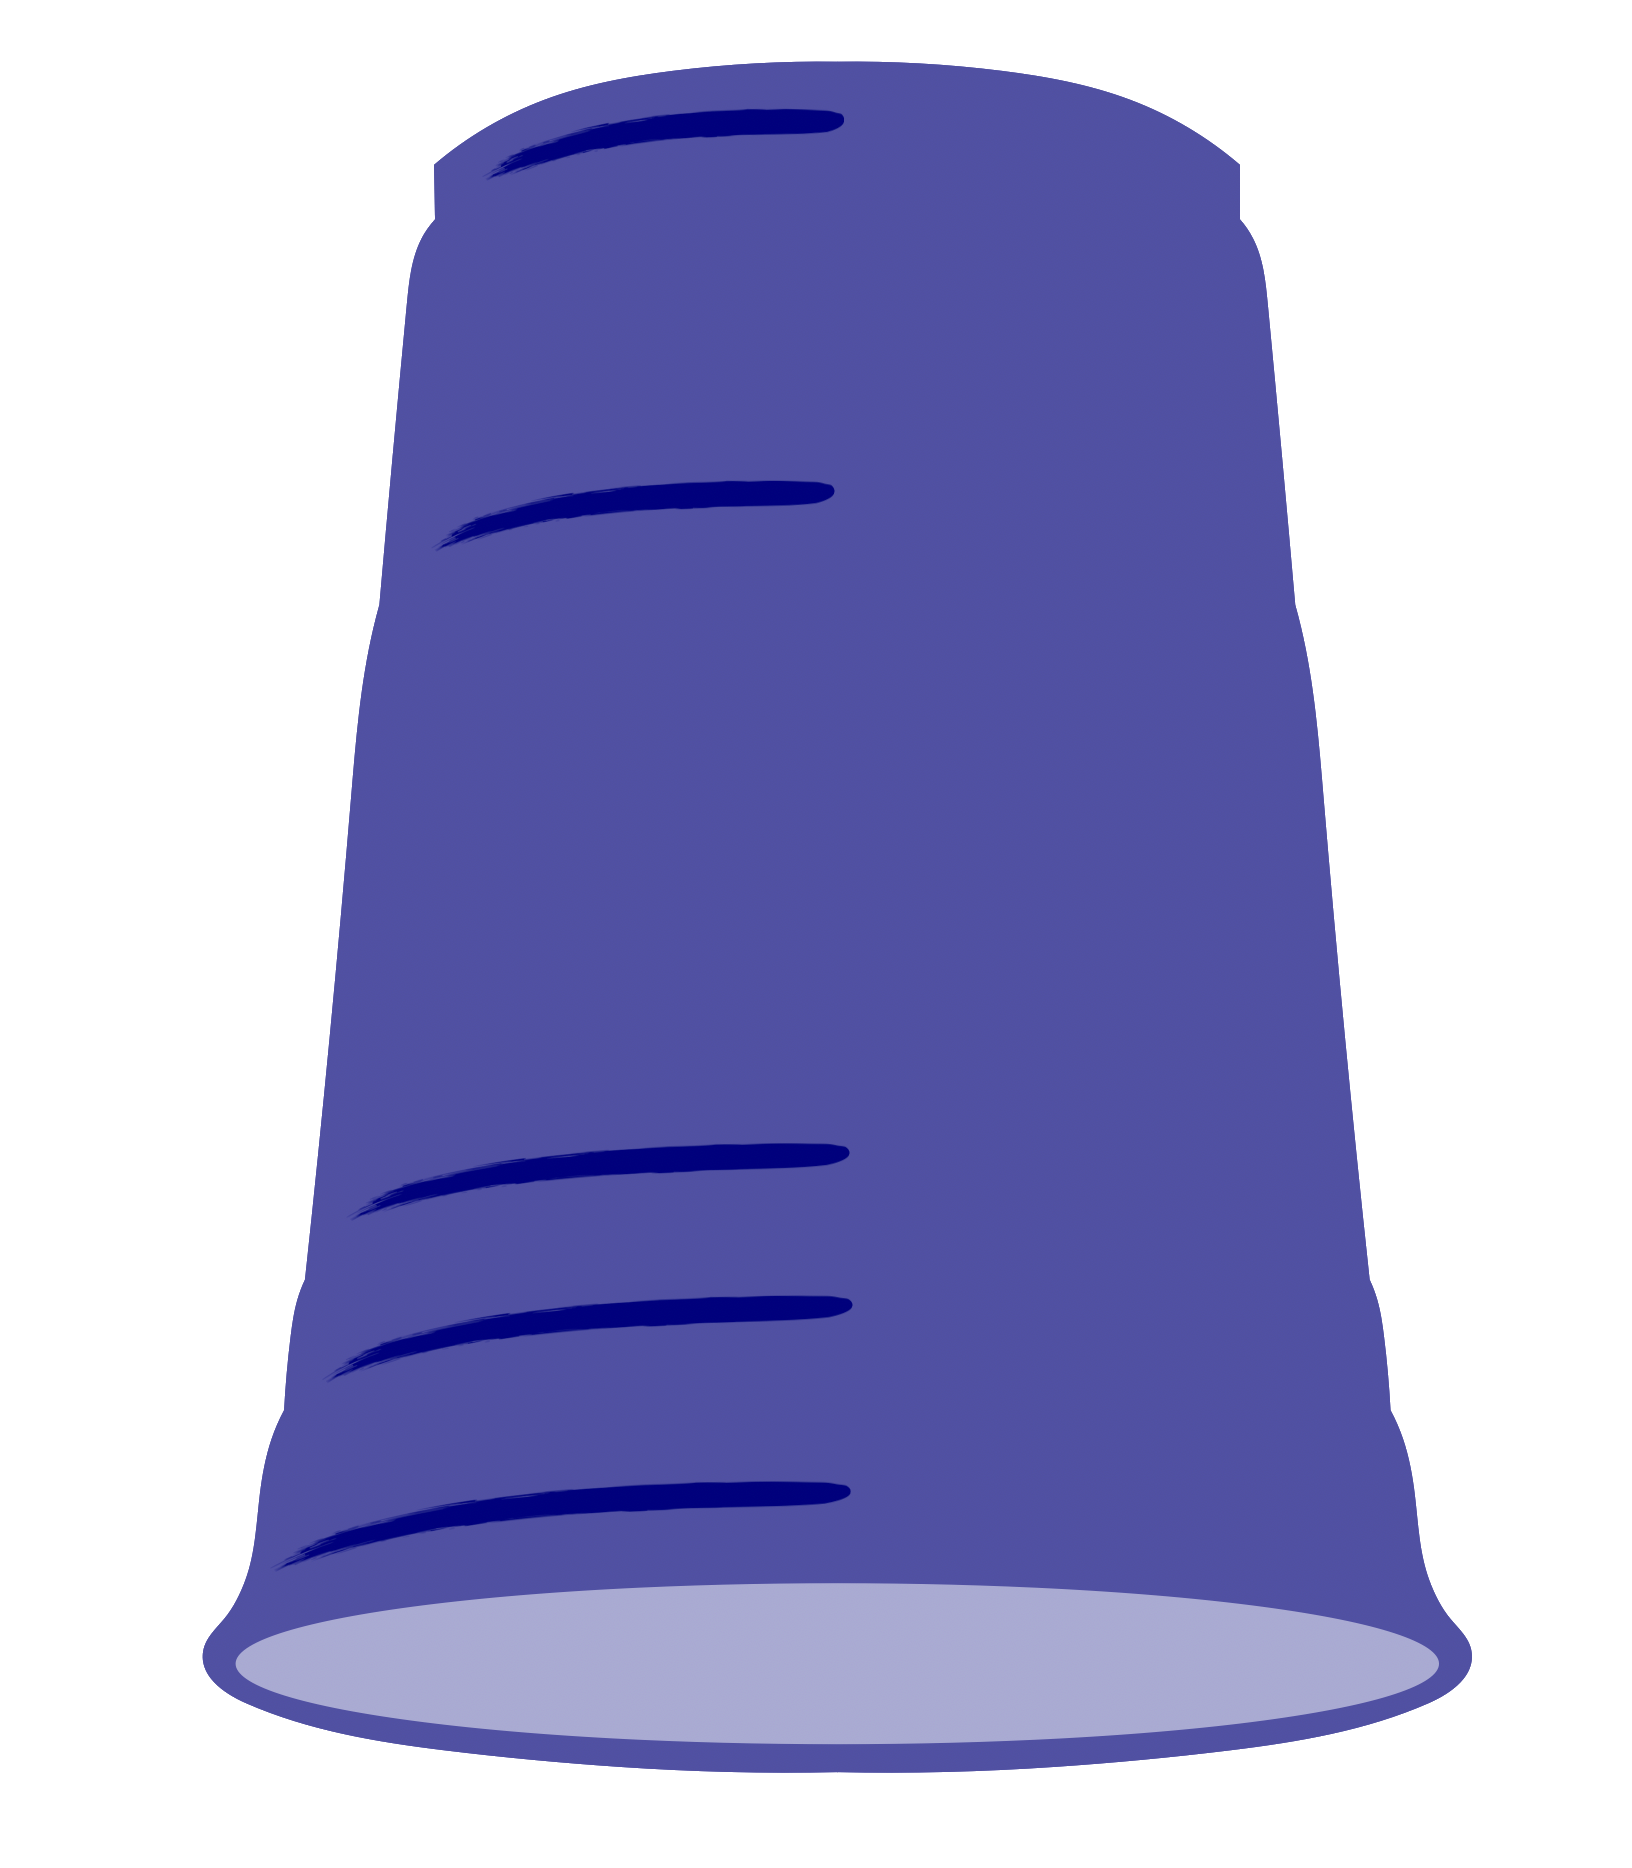
\includegraphics[width=2cm]{cup_up.png}};

				\fill[mid] (0, 4) circle (1);
				\begin{scope}
					\clip (0, 4) circle (1);
					\draw[color=dark, line width=2] (1.1, 4.3) arc[x radius=1.1, y radius=0.2, start angle=0, end angle=180];
					\draw[color=dark, line width=2] (1.1, 3.7) arc[x radius=1.1, y radius=0.2, start angle=0, end angle=180];
				\end{scope}
				\node at (0, 10) {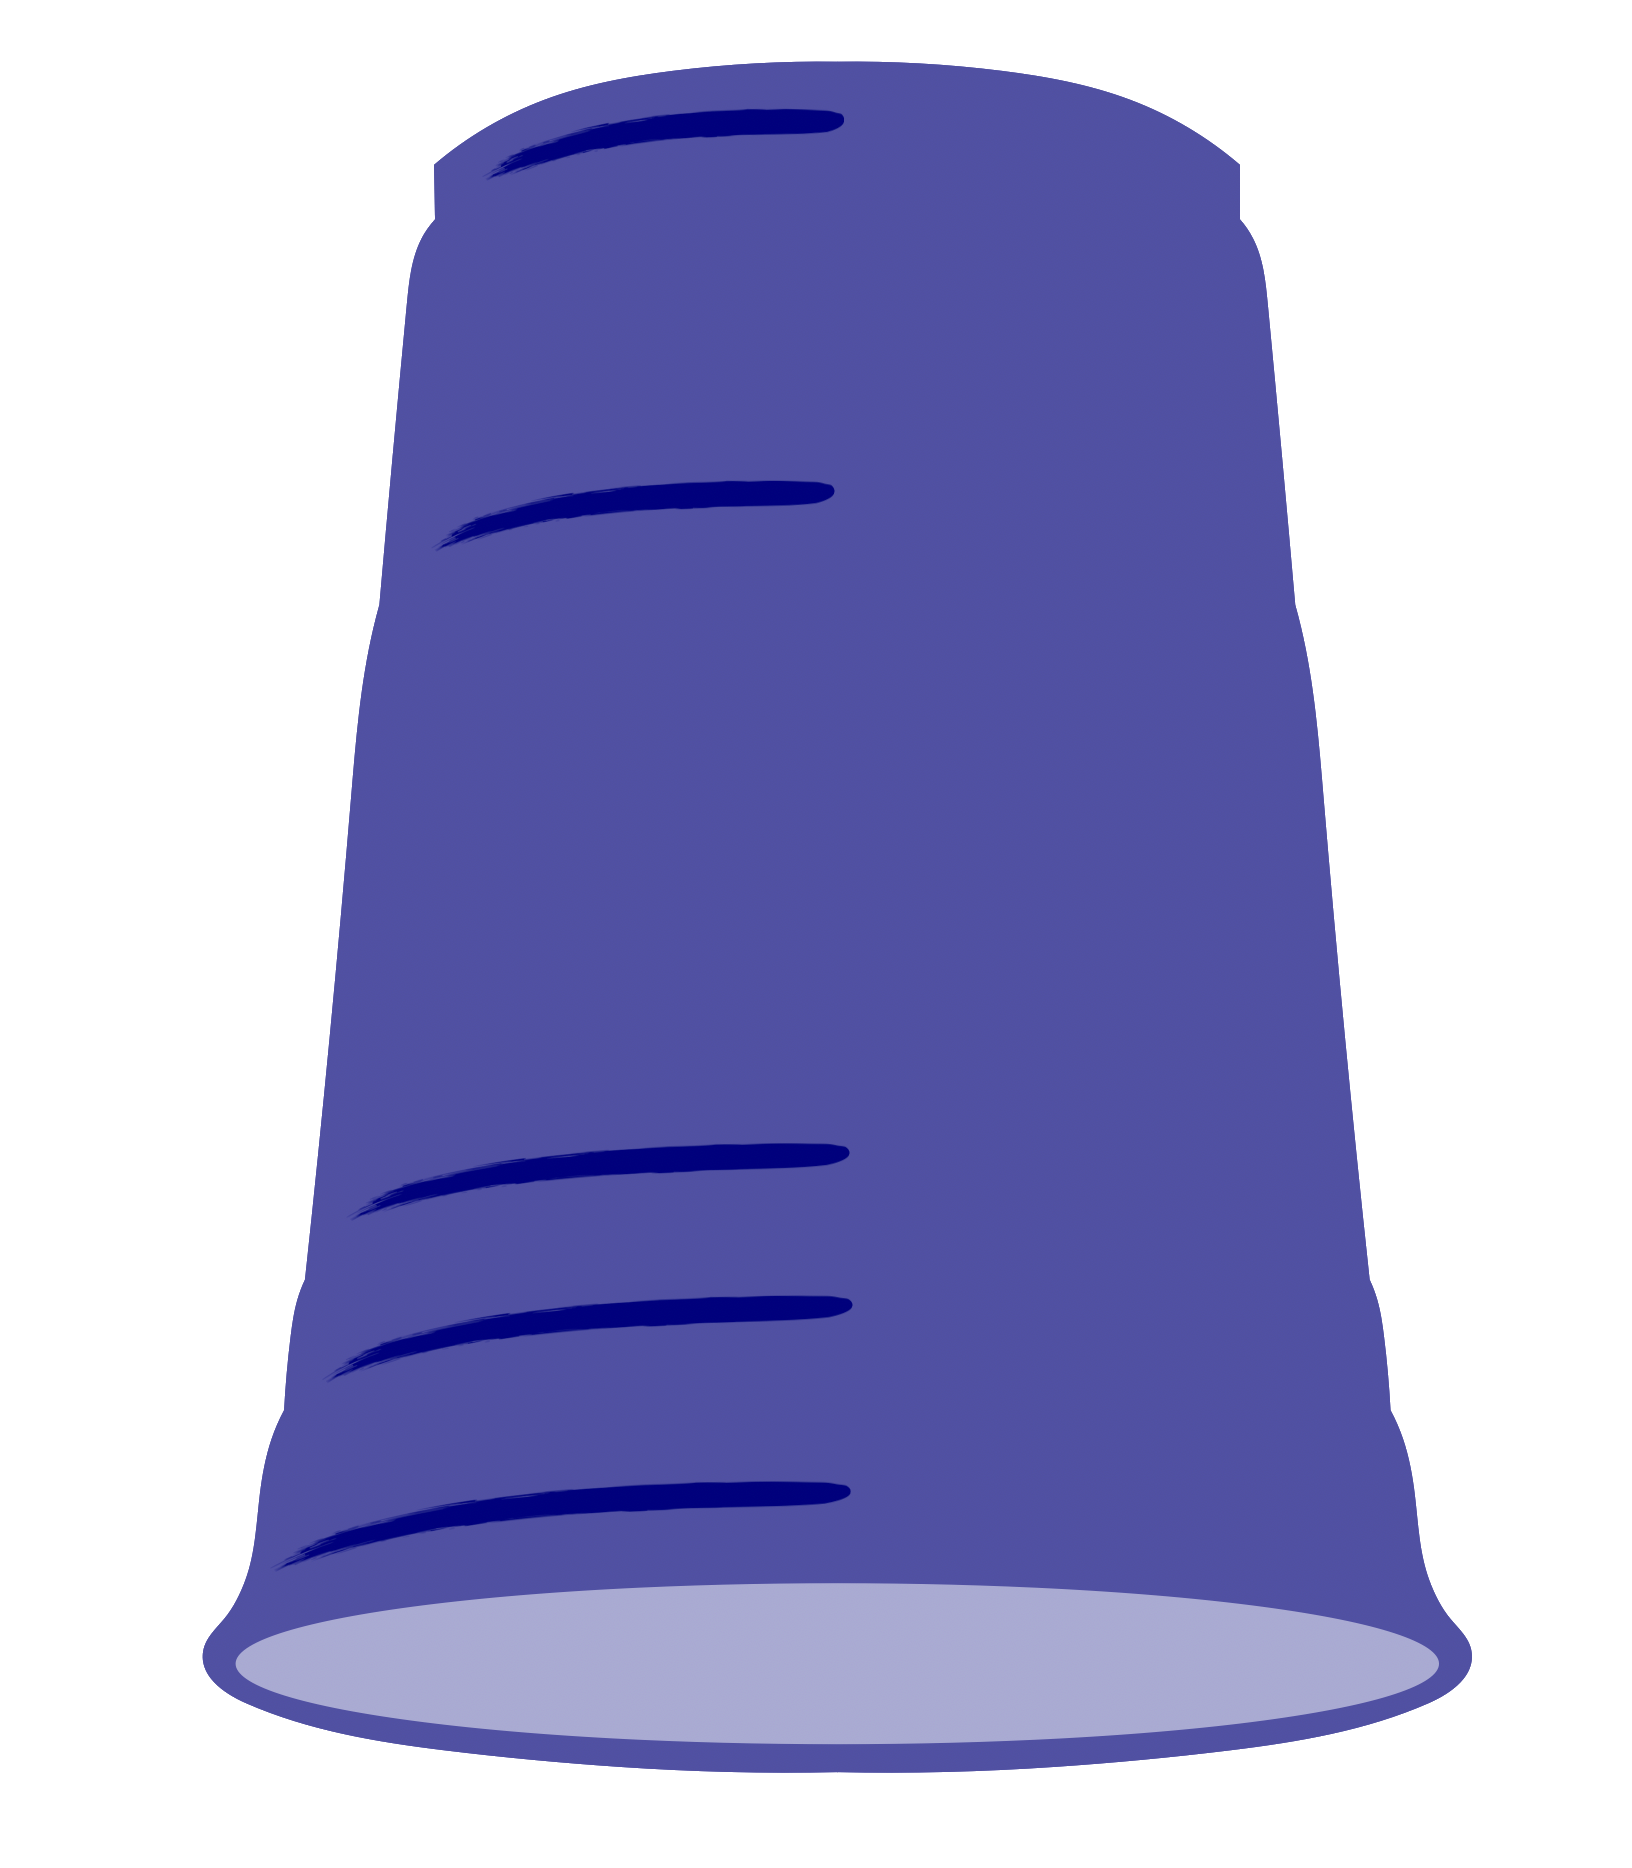
\includegraphics[width=2cm]{cup_up.png}};

				\fill[dark] (+10, 4) circle (1);
				\begin{scope}
					\clip (10, 4) circle (1);
					\draw[color=mid, line width=1] (10, 3) -- (10, 5);
					\draw[color=mid, line width=1] (10.25, 5) arc[x radius=0.3, y radius=1.1, start angle=90, end angle=-90];
					\draw[color=mid, line width=1] (9.75, 5) arc[x radius=0.3, y radius=1.1, start angle=90, end angle=270];
				\end{scope}
				\node at (+10, 10) {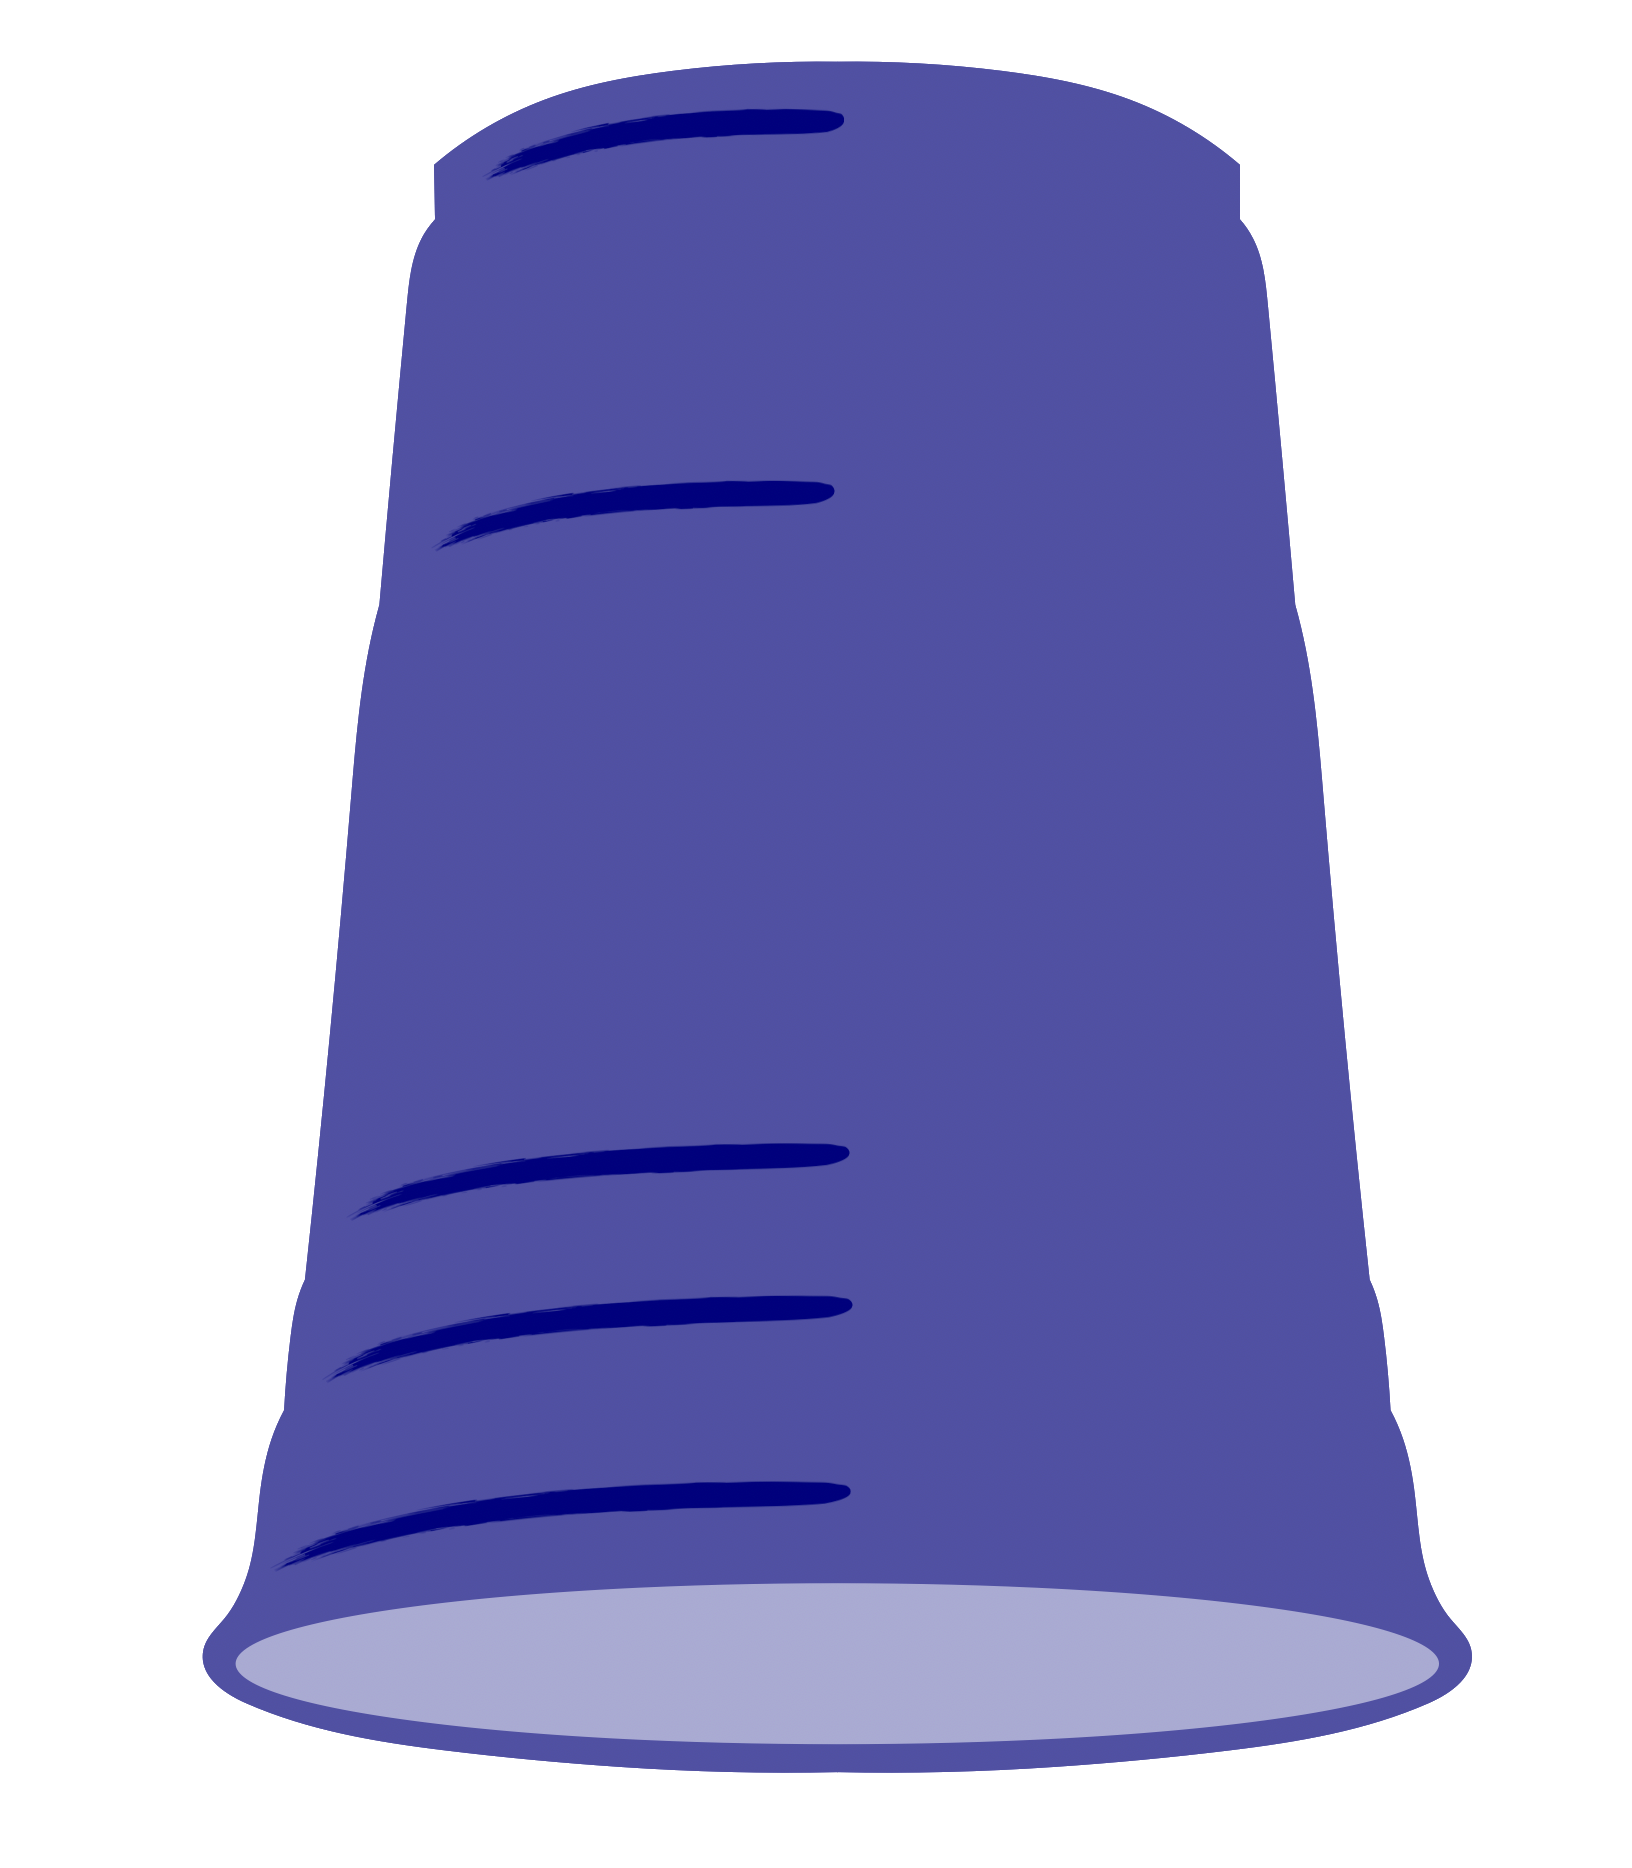
\includegraphics[width=2cm]{cup_up.png}};

			\end{scope}

			% Right
			\begin{scope}[shift={(0, 0)}]

				\draw[white] (-17, 0) rectangle (17, 15);

				\fill[dark] (-10, 4) circle (1);
				\node at (-10, 7) {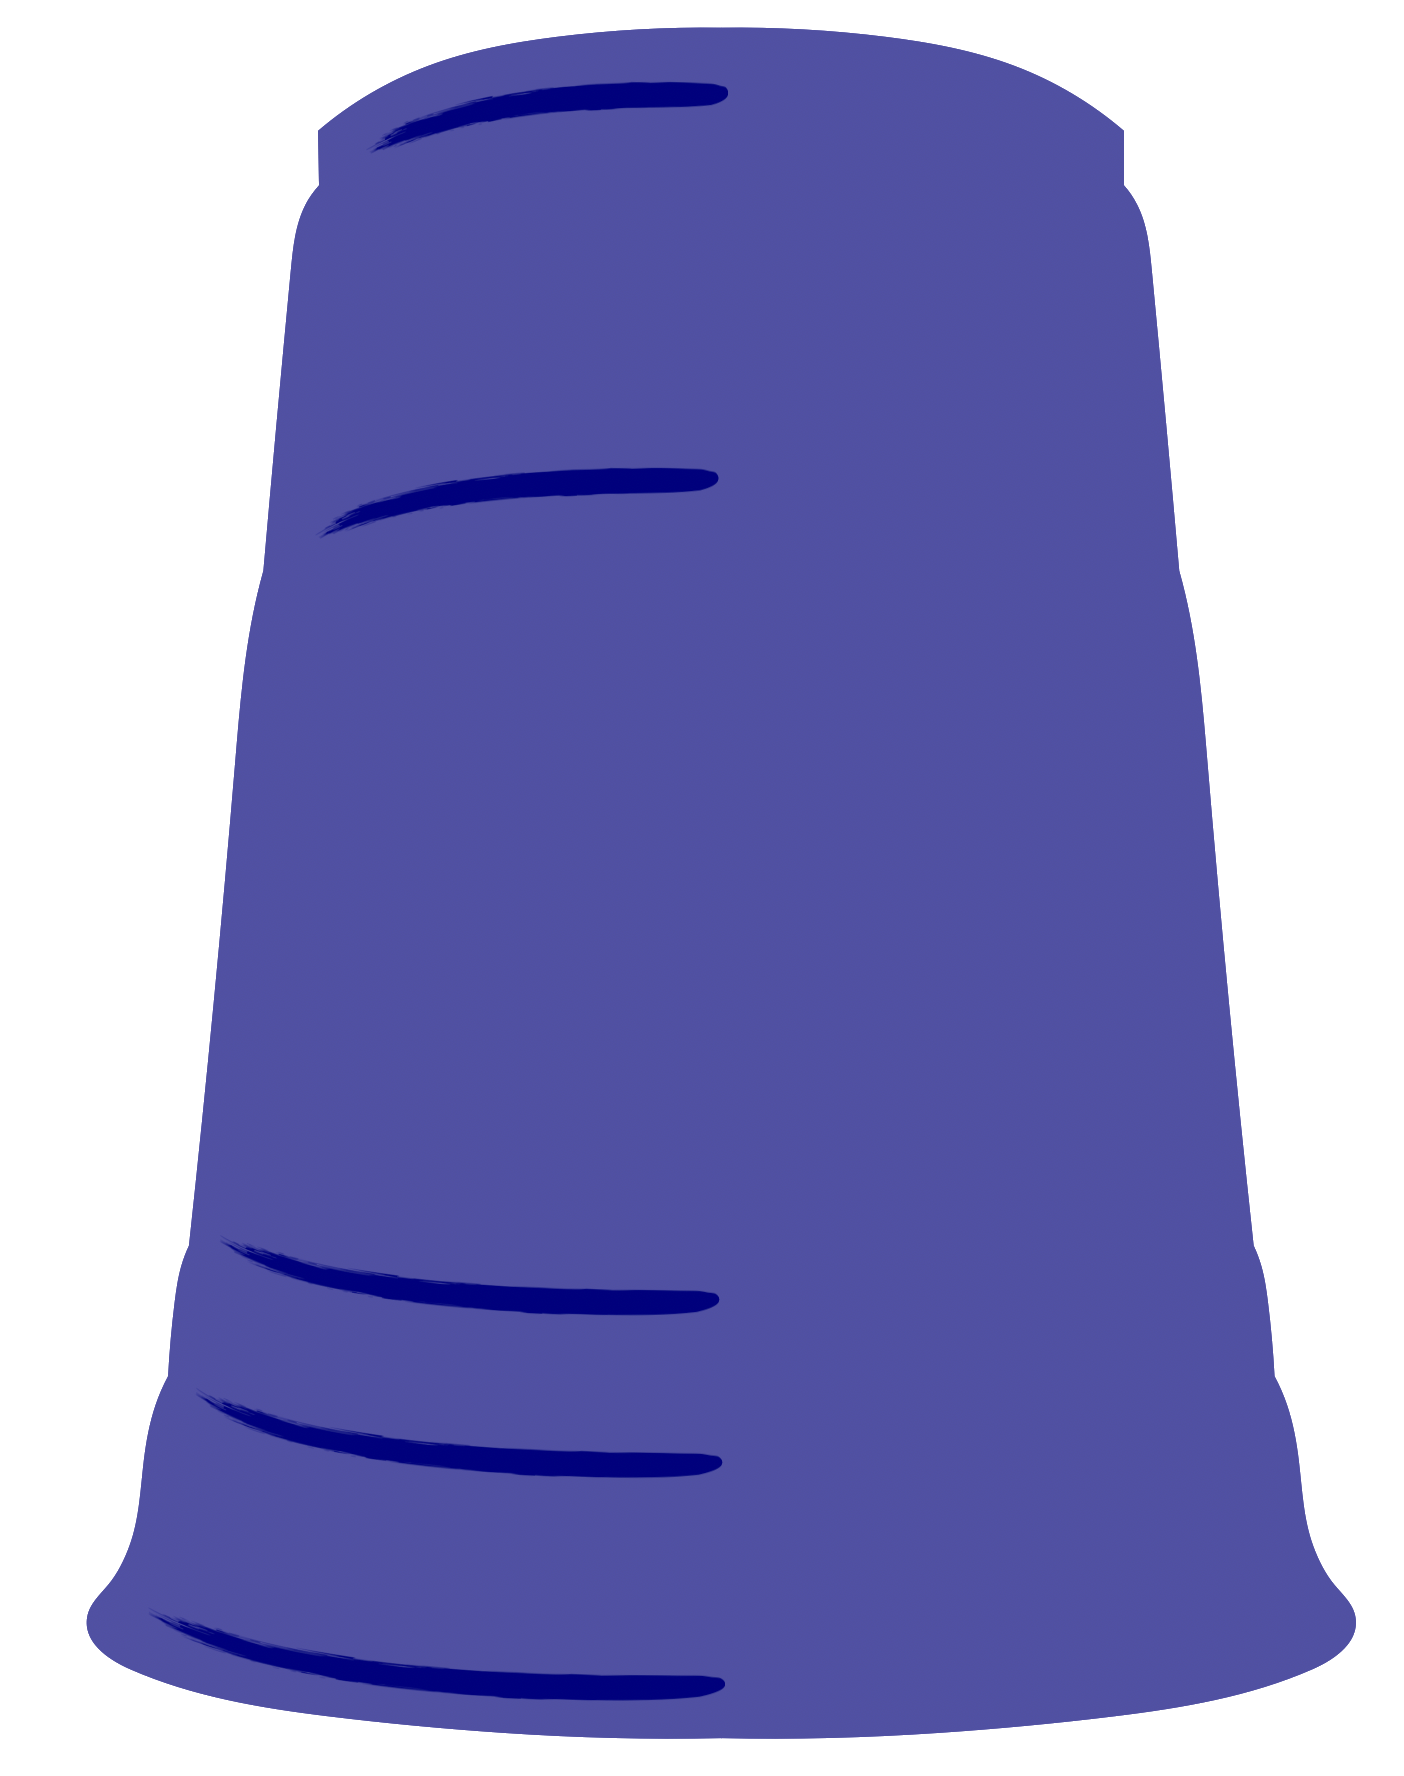
\includegraphics[width=2cm]{cup_down.png}};
				\begin{scope}[scale=0.7, shift={(-17, 3)}, rotate=-5]
					\fill[dark, rounded corners=3] (0, 0) rectangle (10, 6);
					\fill[black] (0, 0.5) rectangle (10, 3.5);
					\node[text=white, align=center, rotate=-5] at (5, 5.2) { \small \textsf{HELLO} };
					\node[text=white, align=center, rotate=-5] at (5, 4.1) { \tiny \textsf{my name is} };
					\node[text=white, align=center, rotate=0] at (5.25, 2) { \large \textsl{Group 1} };
				\end{scope}

				\fill[dark] (0, 4) circle (1);
				\node at (0, 7) {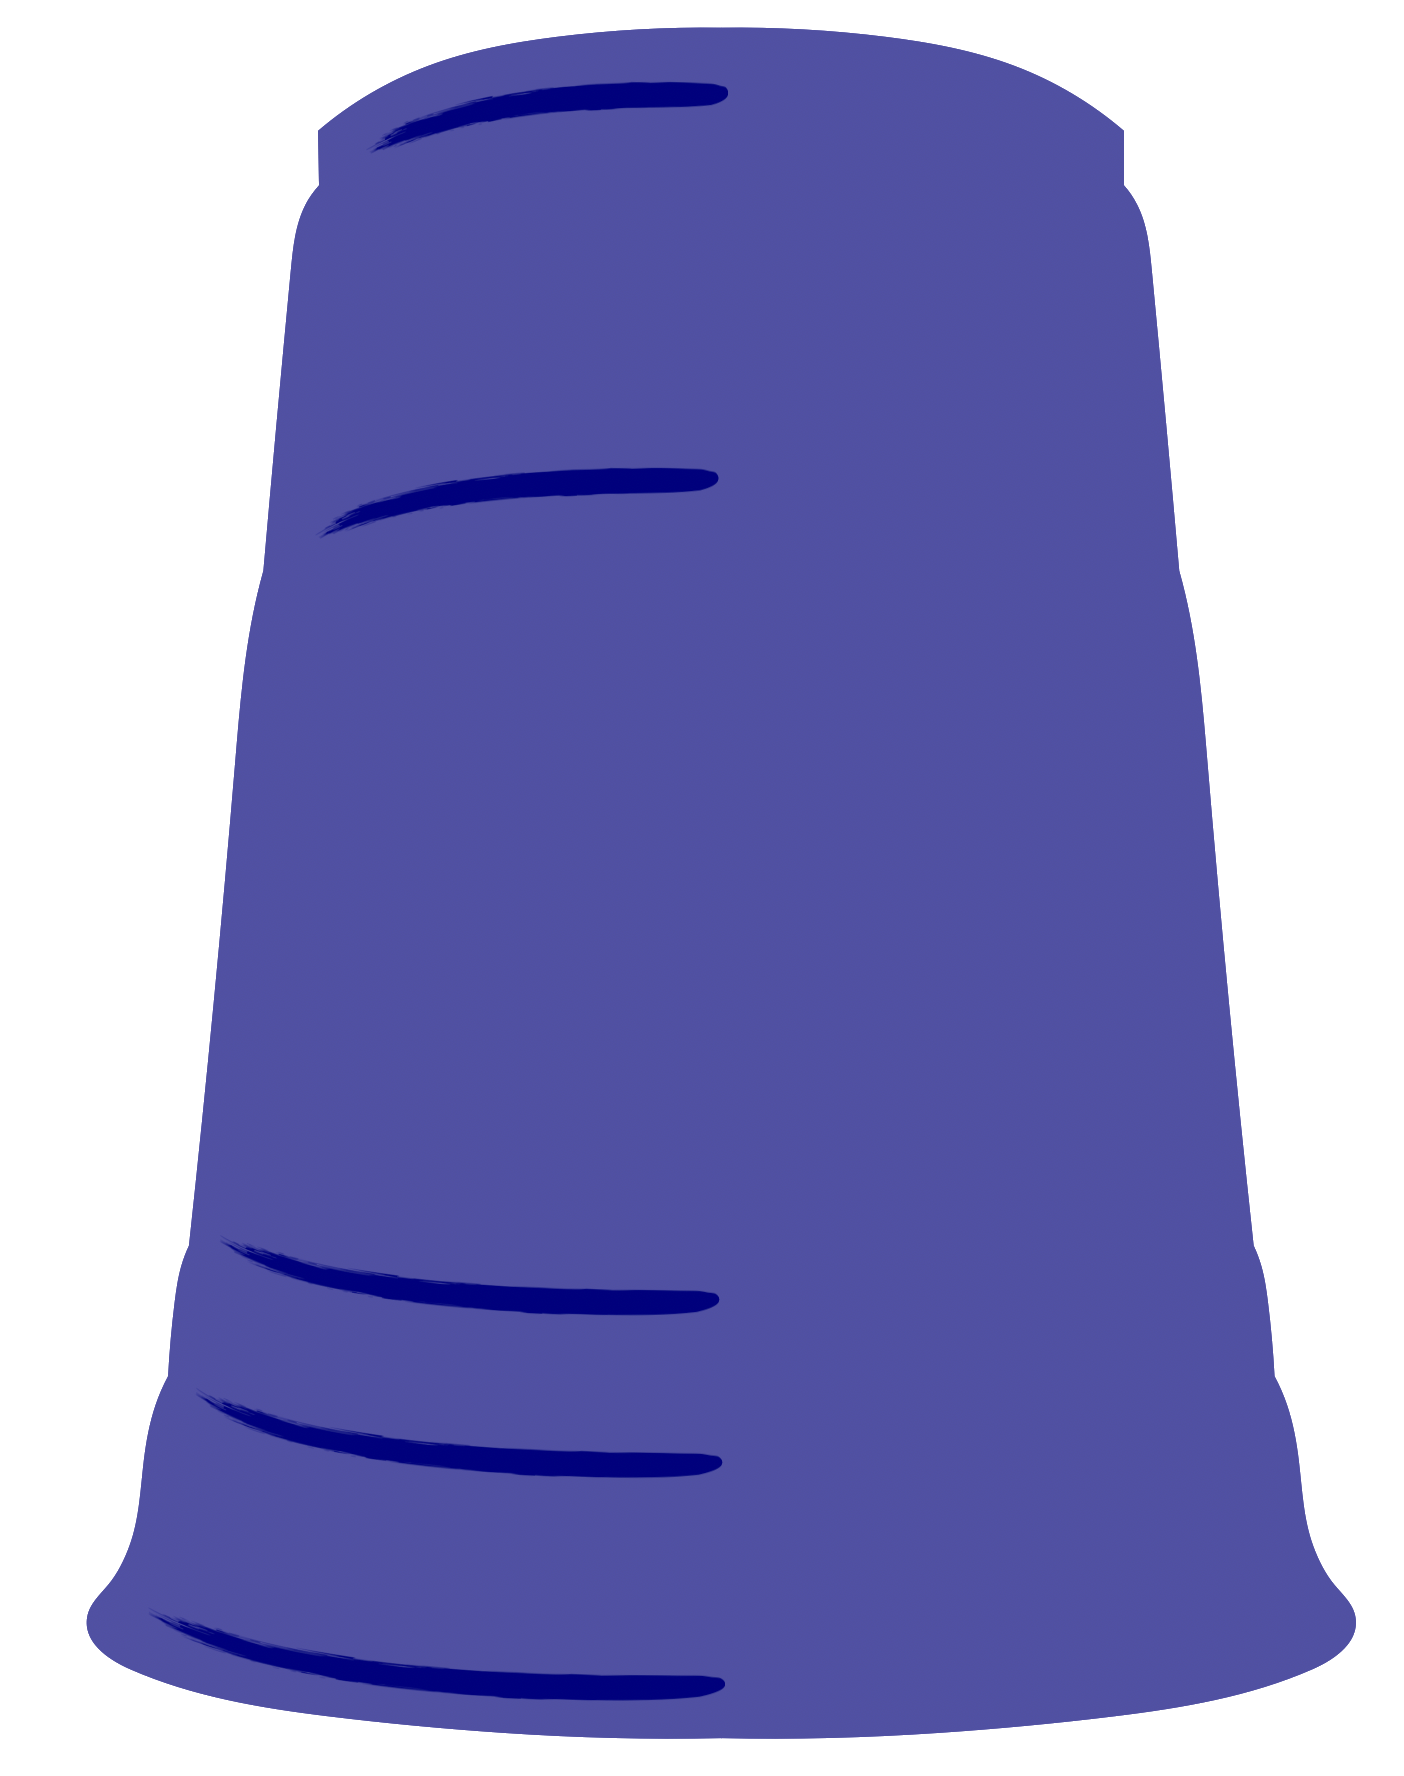
\includegraphics[width=2cm]{cup_down.png}};
				\begin{scope}[scale=0.7, shift={(-2, 3)}, rotate=10]
					\fill[dark, rounded corners=3] (0, 0) rectangle (10, 6);
					\fill[black] (0, 0.5) rectangle (10, 3.5);
					\node[text=white, align=center, rotate=10] at (5, 5.2) { \small \textsf{HELLO} };
					\node[text=white, align=center, rotate=10] at (5, 4.1) { \tiny \textsf{my name is } };
					\node[text=white, align=center, rotate=7] at (5.25, 2) { \large \textsl{Group 2} };
				\end{scope}

				\fill[dark] (+10, 4) circle (1);
				\node at (+10, 7) {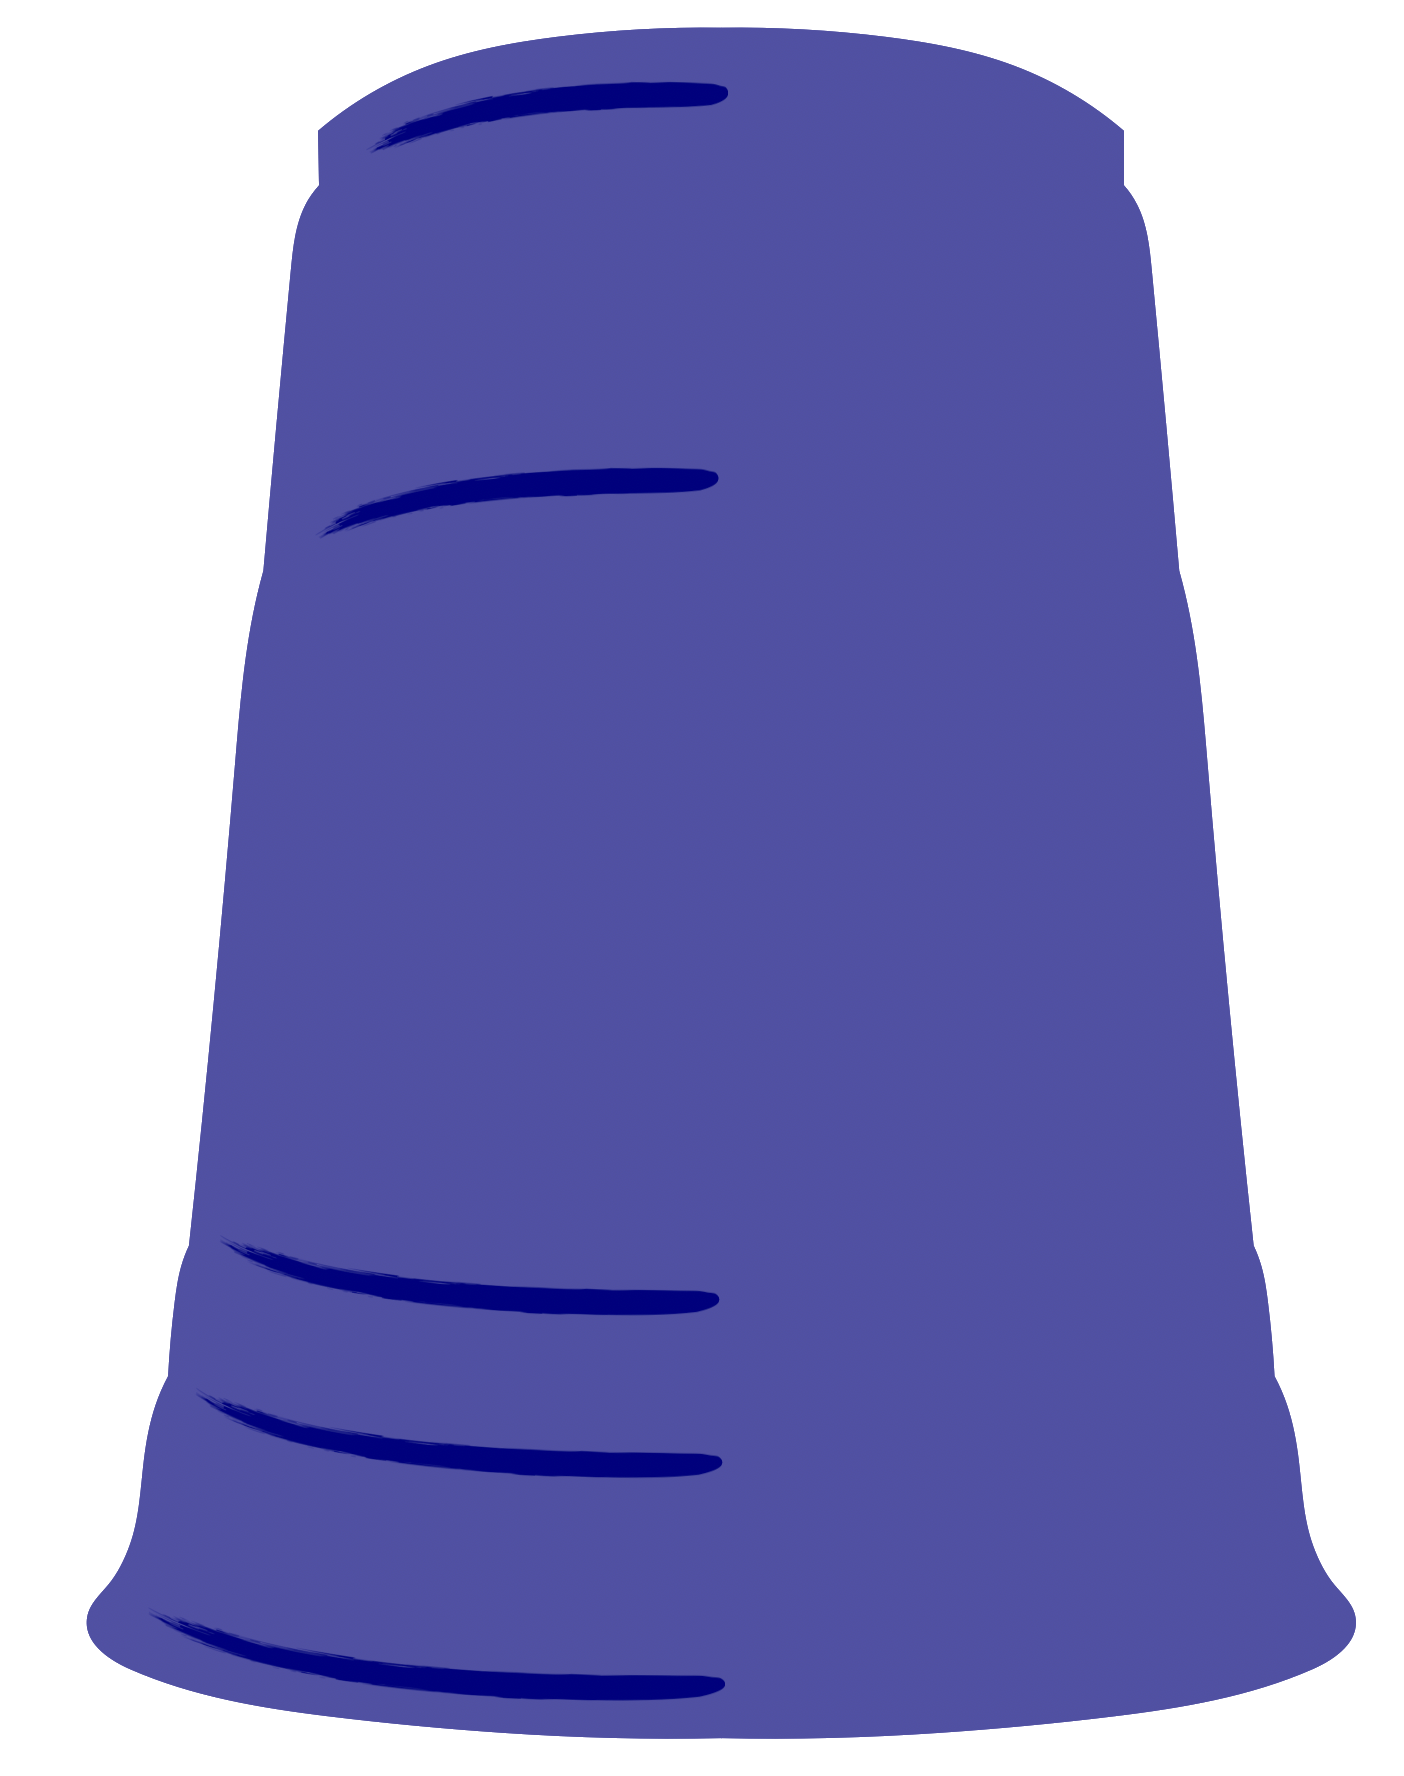
\includegraphics[width=2cm]{cup_down.png}};
				\begin{scope}[scale=0.7, shift={(12, 3)}, rotate=1]
					\fill[dark, rounded corners=3] (0, 0) rectangle (10, 6);
					\fill[black] (0, 0.5) rectangle (10, 3.5);
					\node[text=white, align=center, rotate=1] at (5, 5.2) { \small \textsf{HELLO} };
					\node[text=white, align=center, rotate=1] at (5, 4.1) { \tiny \textsf{my name is } };
					\node[text=white, align=center, rotate=1] at (5.25, 2) { \large \textsl{Group 3} };
				\end{scope}
			\end{scope}
		\end{tikzpicture}
	\end{adjustbox}
\end{frame}

\begin{frame}{Exchangeability \parencite{definettiTheoryProbability1974}\footnote{figures adapted from \href{https://betanalpha.github.io/assets/case_studies/hierarchical_modeling.html}{Michael Betancourt (CC-BY-SA-4.0)}.}}
	\begin{adjustbox}{max width=1.0\textwidth}
		\begin{tikzpicture}[scale=0.3, thick]


			\draw[white] (-17, -3) rectangle (17, 15);

			\fill[dark] (-10, 4) circle (1);
			\node at (-10, 7) {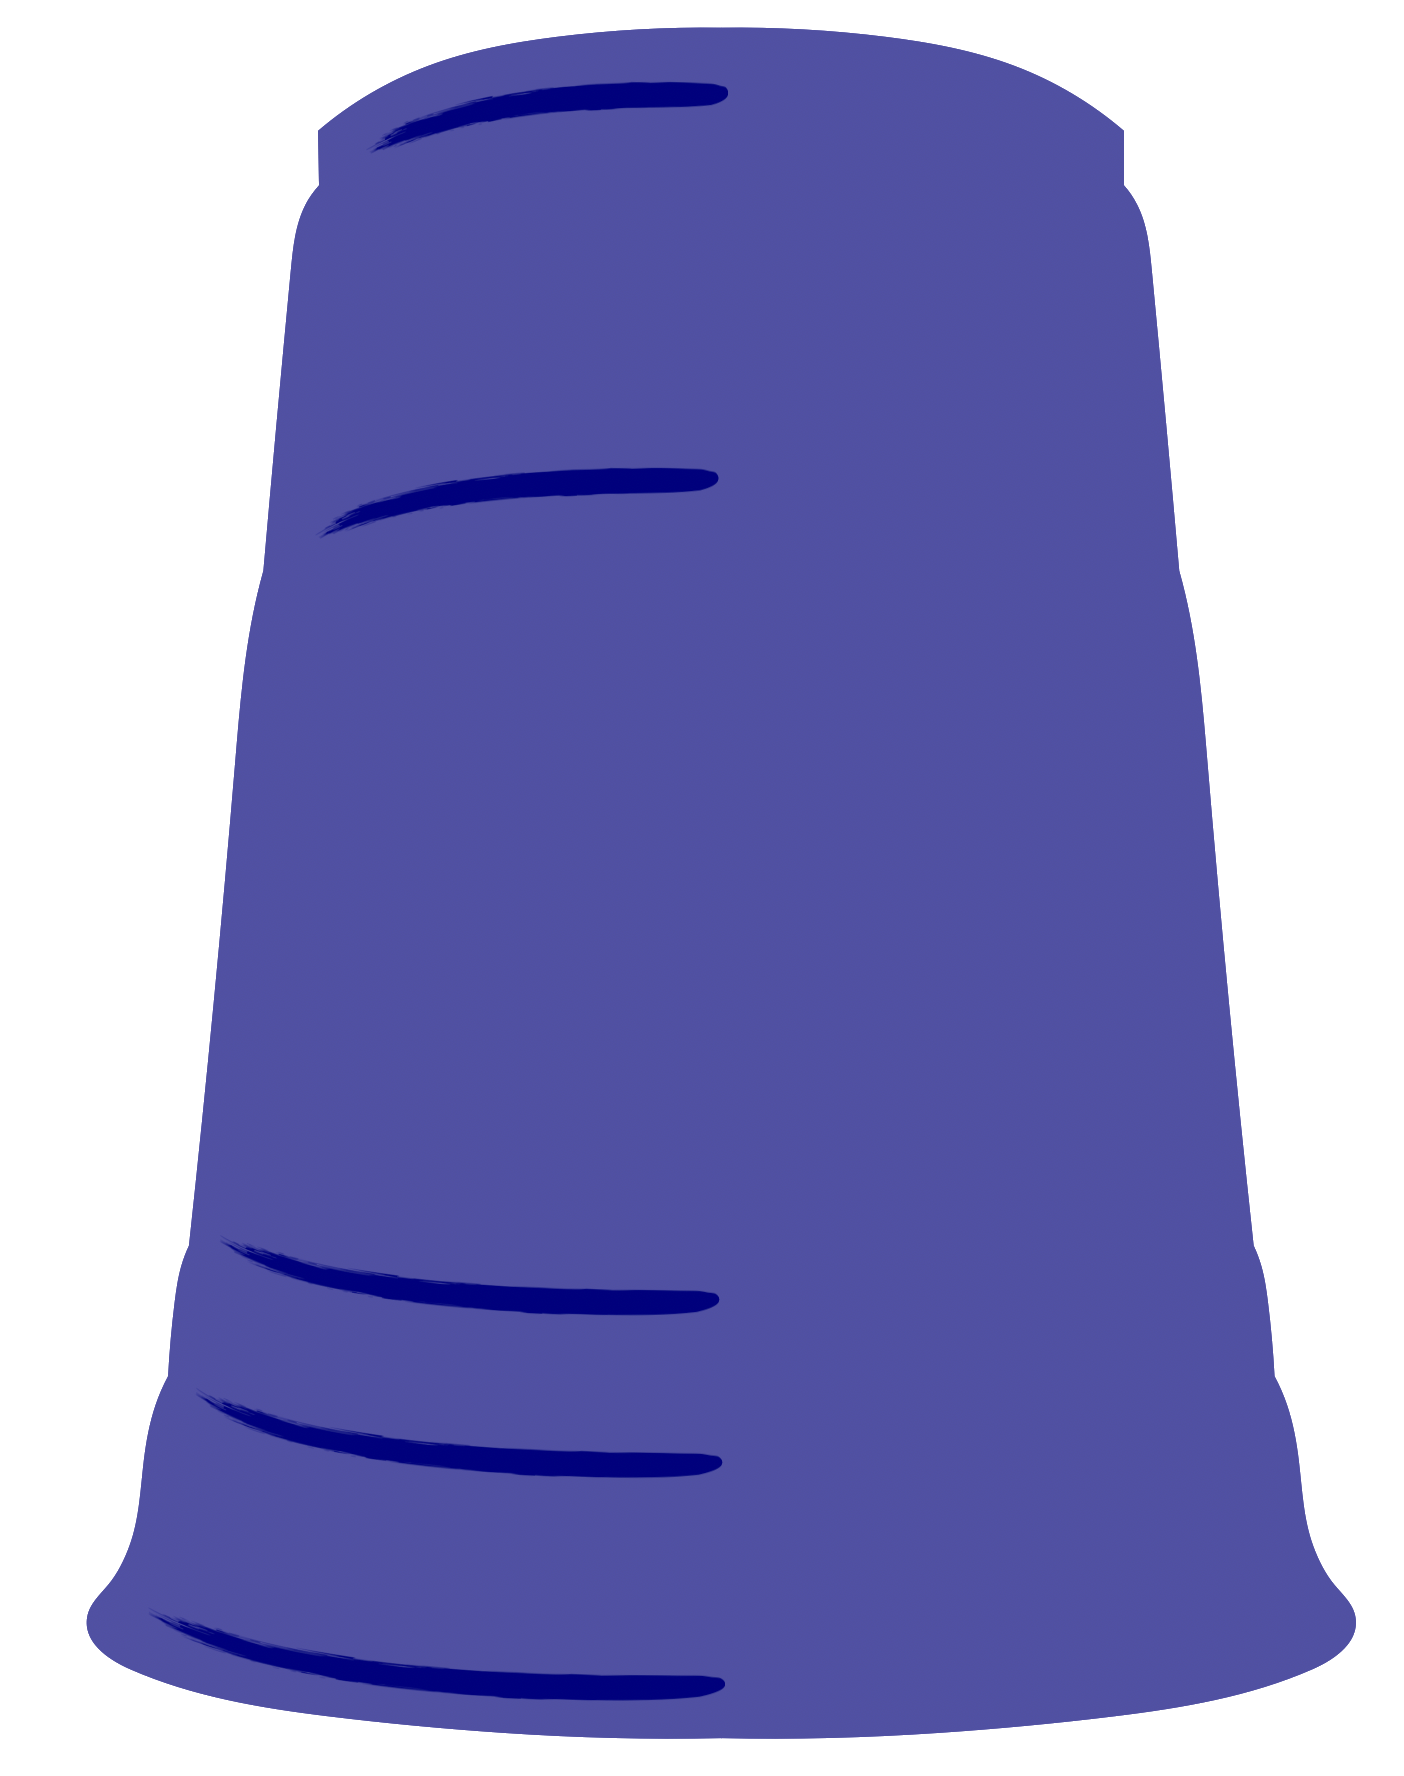
\includegraphics[width=2cm]{cup_down.png}};

			% Left
			\begin{scope}[scale=0.7, shift={(-17, 3)}, rotate=-5]
				\fill[dark, rounded corners=3] (0, 0) rectangle (10, 6);
				\fill[black] (0, 0.5) rectangle (10, 3.5);
				\node[text=white, align=center, rotate=-5] at (5, 5.2) { \small \textsf{HELLO} };
				\node[text=white, align=center, rotate=-5] at (5, 4.1) { \tiny \textsf{my name is } };
				\node[text=white, align=center, rotate=0] at (5.25, 2) { \large \textsl{Group 1} };
			\end{scope}

			\fill[dark] (0, 4) circle (1);
			\node at (0, 7) {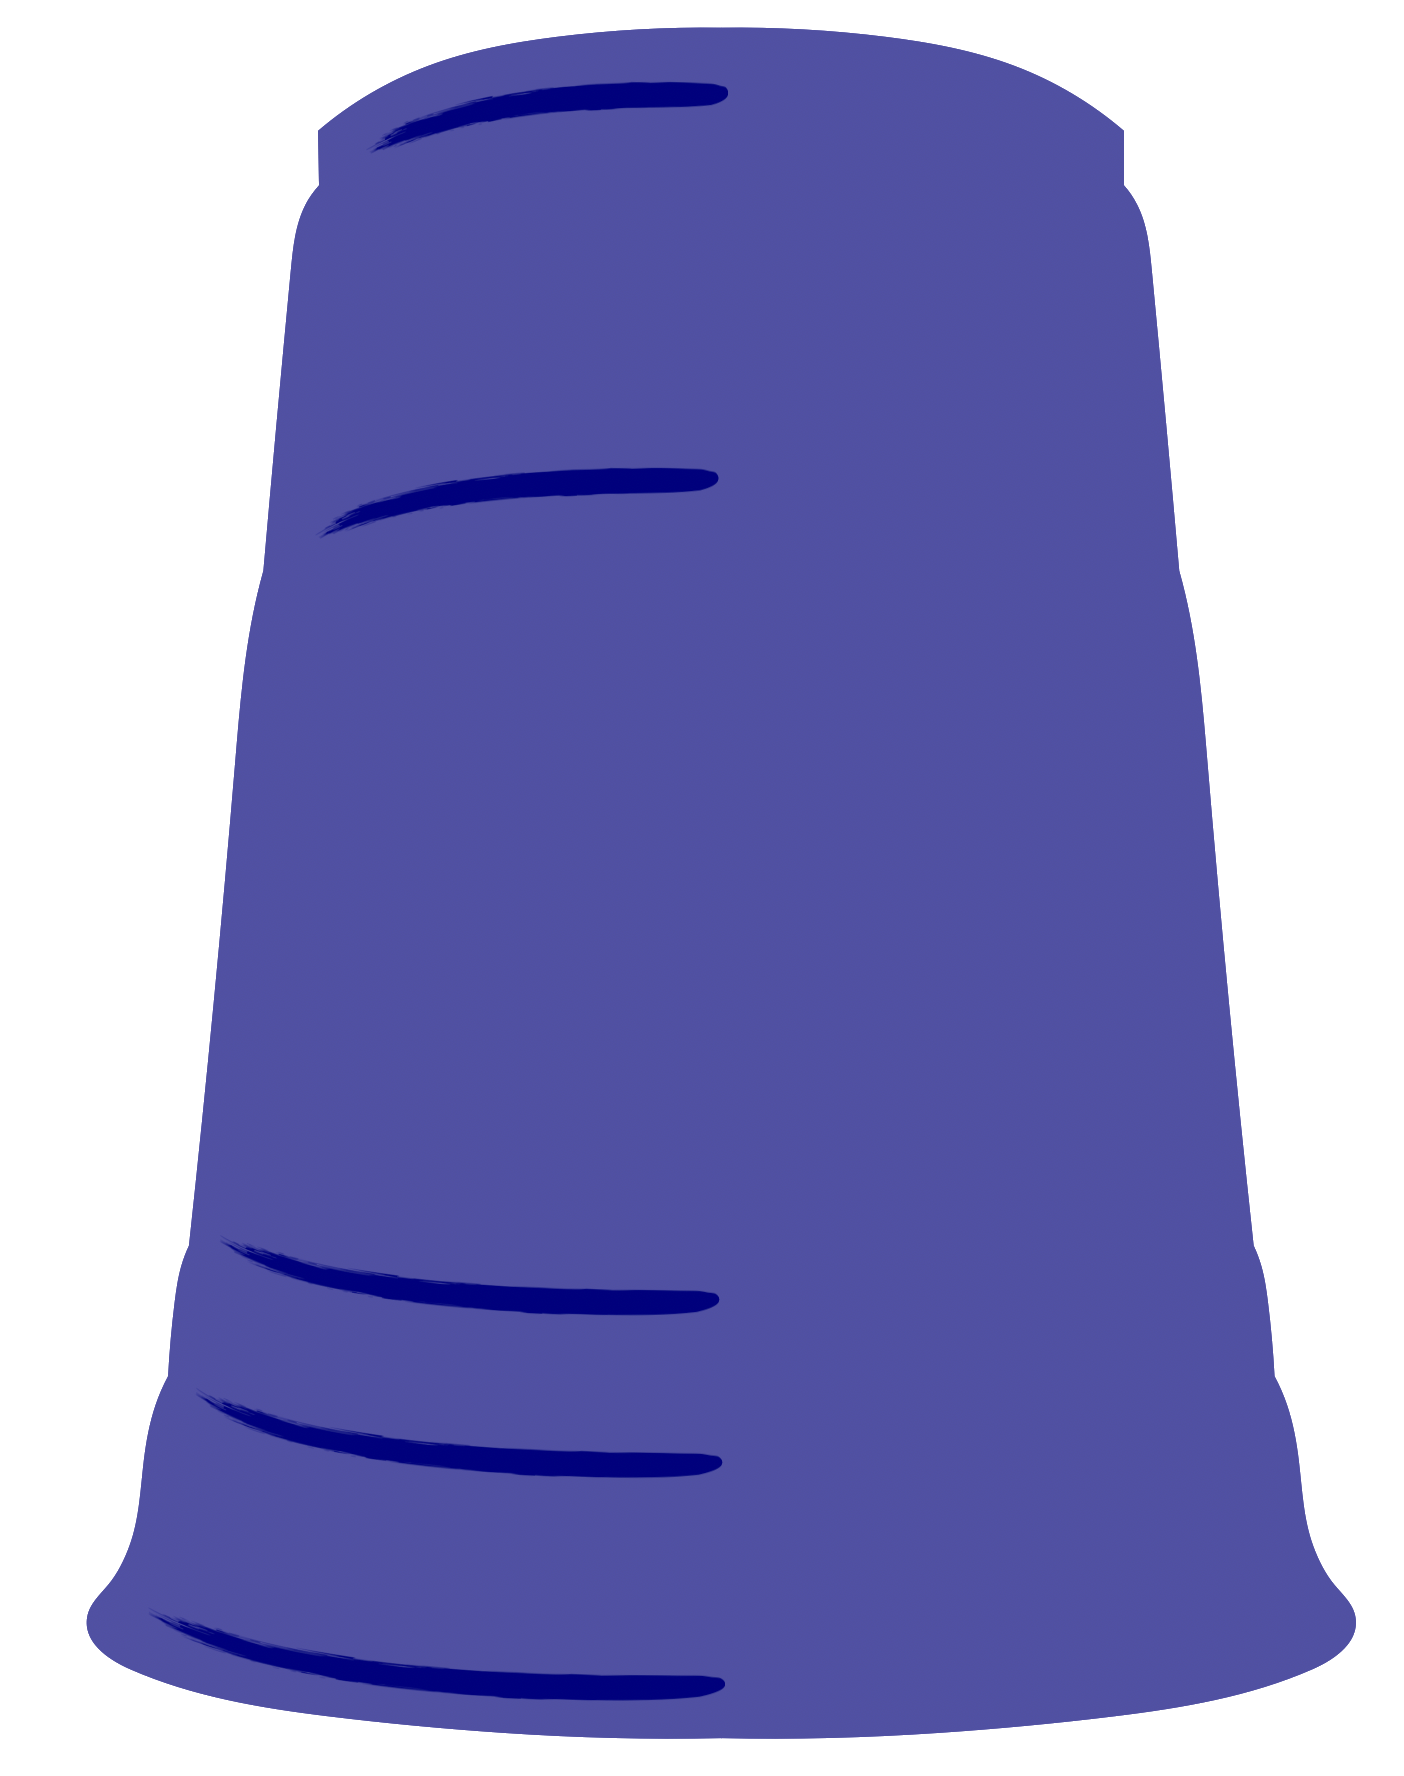
\includegraphics[width=2cm]{cup_down.png}};

			\begin{scope}[scale=0.7, shift={(-2, 3)}, rotate=10]
				\fill[dark, rounded corners=3] (0, 0) rectangle (10, 6);
				\fill[black] (0, 0.5) rectangle (10, 3.5);
				\node[text=white, align=center, rotate=10] at (5, 5.2) { \small \textsf{HELLO} };
				\node[text=white, align=center, rotate=10] at (5, 4.1) { \tiny \textsf{my name is } };
				\node[text=white, align=center, rotate=7] at (5.25, 2) { \large \textsl{Group 2} };
			\end{scope}

			\fill[dark] (+10, 4) circle (1);
			\node at (+10, 7) {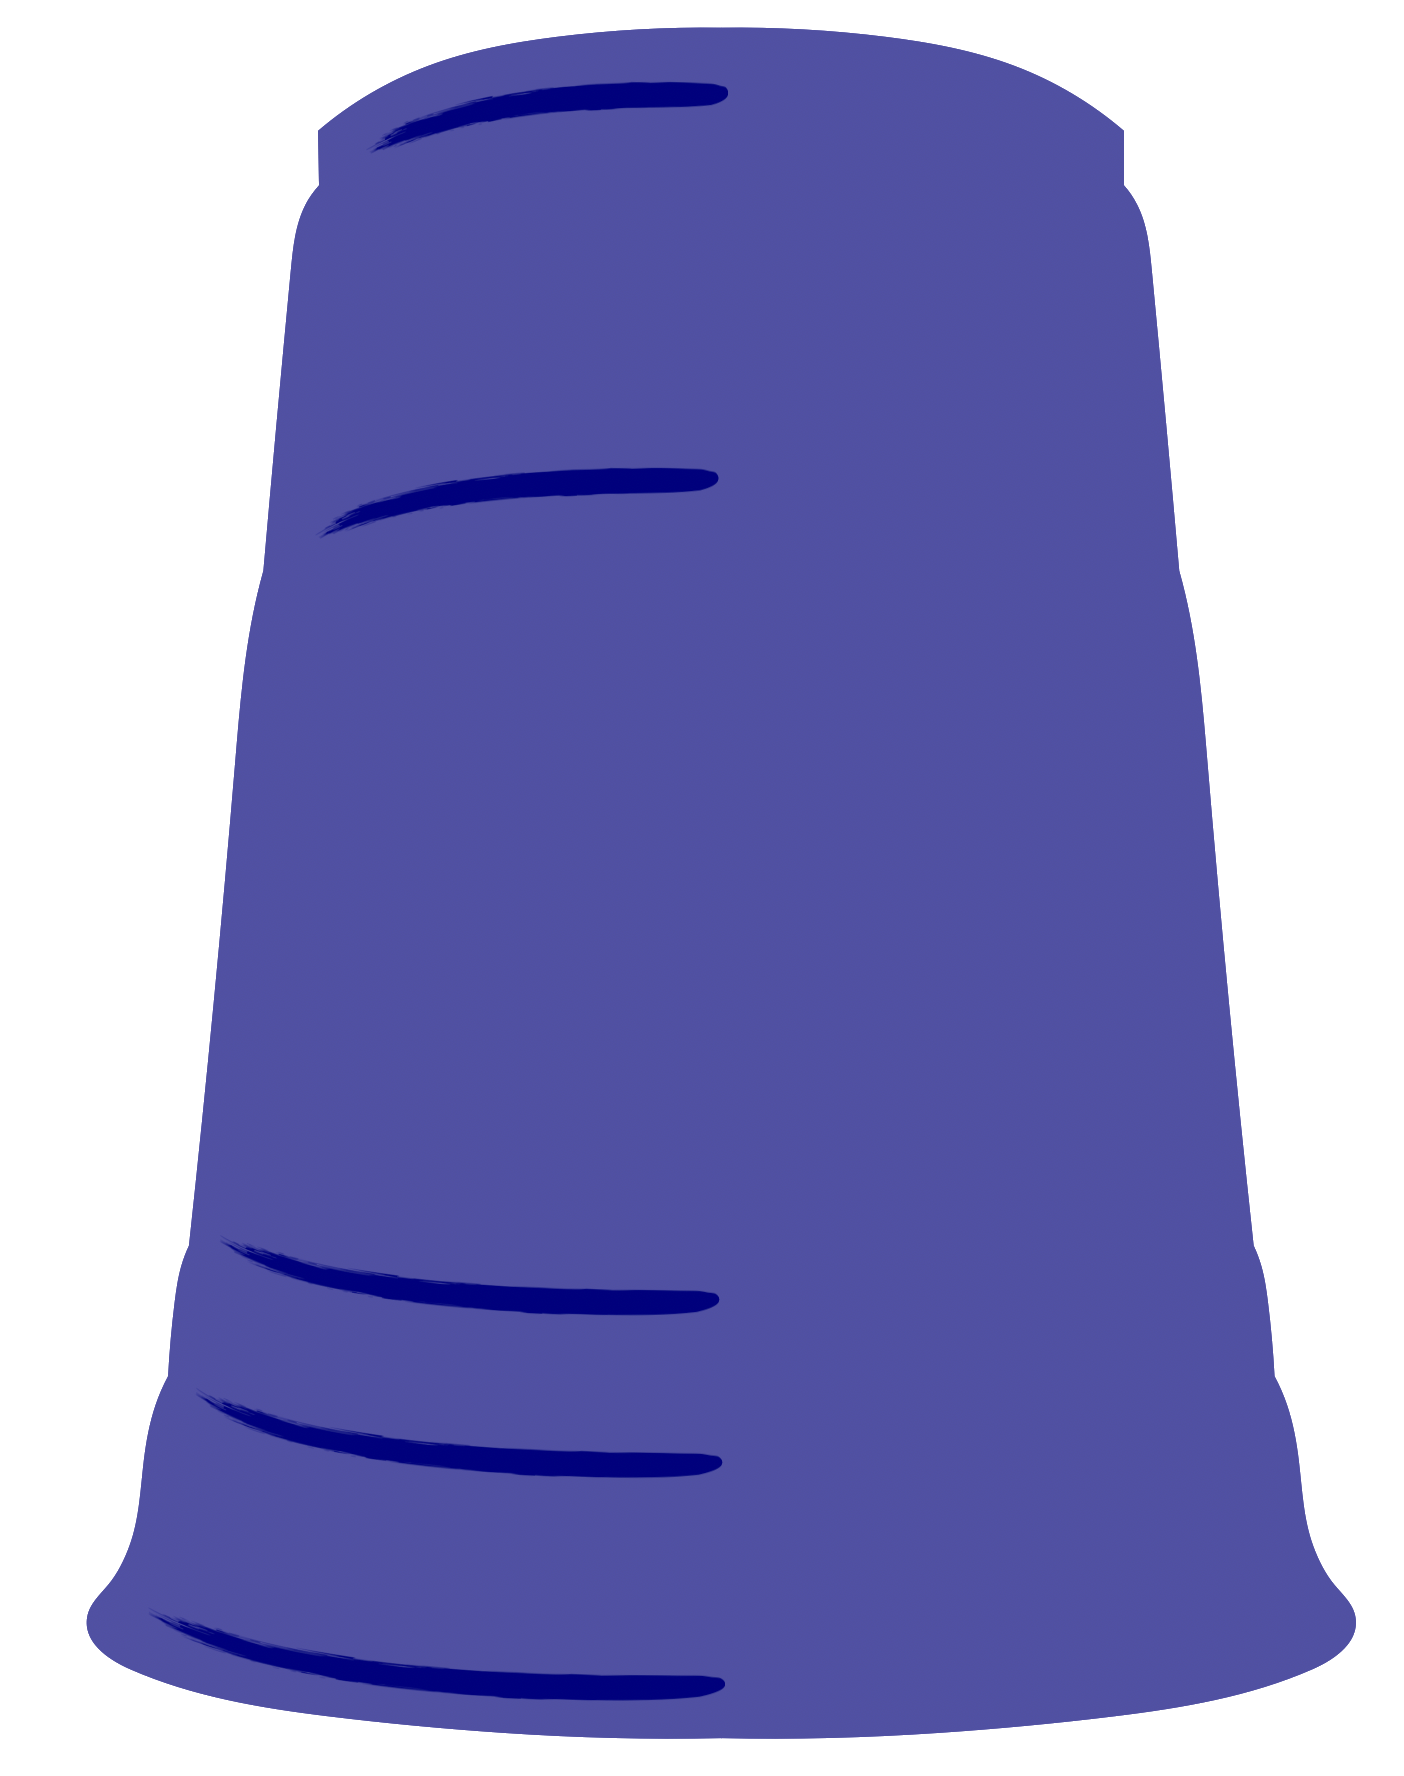
\includegraphics[width=2cm]{cup_down.png}};

			\begin{scope}[scale=0.7, shift={(12, 3)}, rotate=1]
				\fill[dark, rounded corners=3] (0, 0) rectangle (10, 6);
				\fill[black] (0, 0.5) rectangle (10, 3.5);
				\node[text=white, align=center, rotate=1] at (5, 5.2) { \small \textsf{HELLO} };
				\node[text=white, align=center, rotate=1] at (5, 4.1) { \tiny \textsf{my name is } };
				\node[text=white, align=center, rotate=1] at (5.25, 2) { \large \textsl{Group 3} };
			\end{scope}

			\pgfmathsetmacro{\r}{10}
			\pgfmathsetmacro{\start}{160}
			\pgfmathsetmacro{\stop}{20}

			\draw[dark, <->, >=stealth] ({0 + \r * cos(\start)}, {8 + \r * sin(\start)})
			arc[x radius = \r, y radius = 3, start angle=\start, end angle= \stop];

			\pgfmathsetmacro{\r}{3}
			\pgfmathsetmacro{\start}{160}
			\pgfmathsetmacro{\stop}{20}

			\draw[dark, <->, >=stealth] ({-5 + \r * cos(\start)}, {10 + \r * sin(\start)})
			arc[x radius = \r, y radius = 0.75, start angle=\start, end angle= \stop];

			\draw[dark, <->, >=stealth] ({5 + \r * cos(\start)}, {10 + \r * sin(\start)})
			arc[x radius = \r, y radius = 0.75, start angle=\start, end angle= \stop];

			% Right
			\begin{scope}[shift={(36, 0)}]

				\draw[white] (-17, -3) rectangle (17, 15);

				\fill[dark] (-10, 4) circle (1);
				\node at (-10, 7) {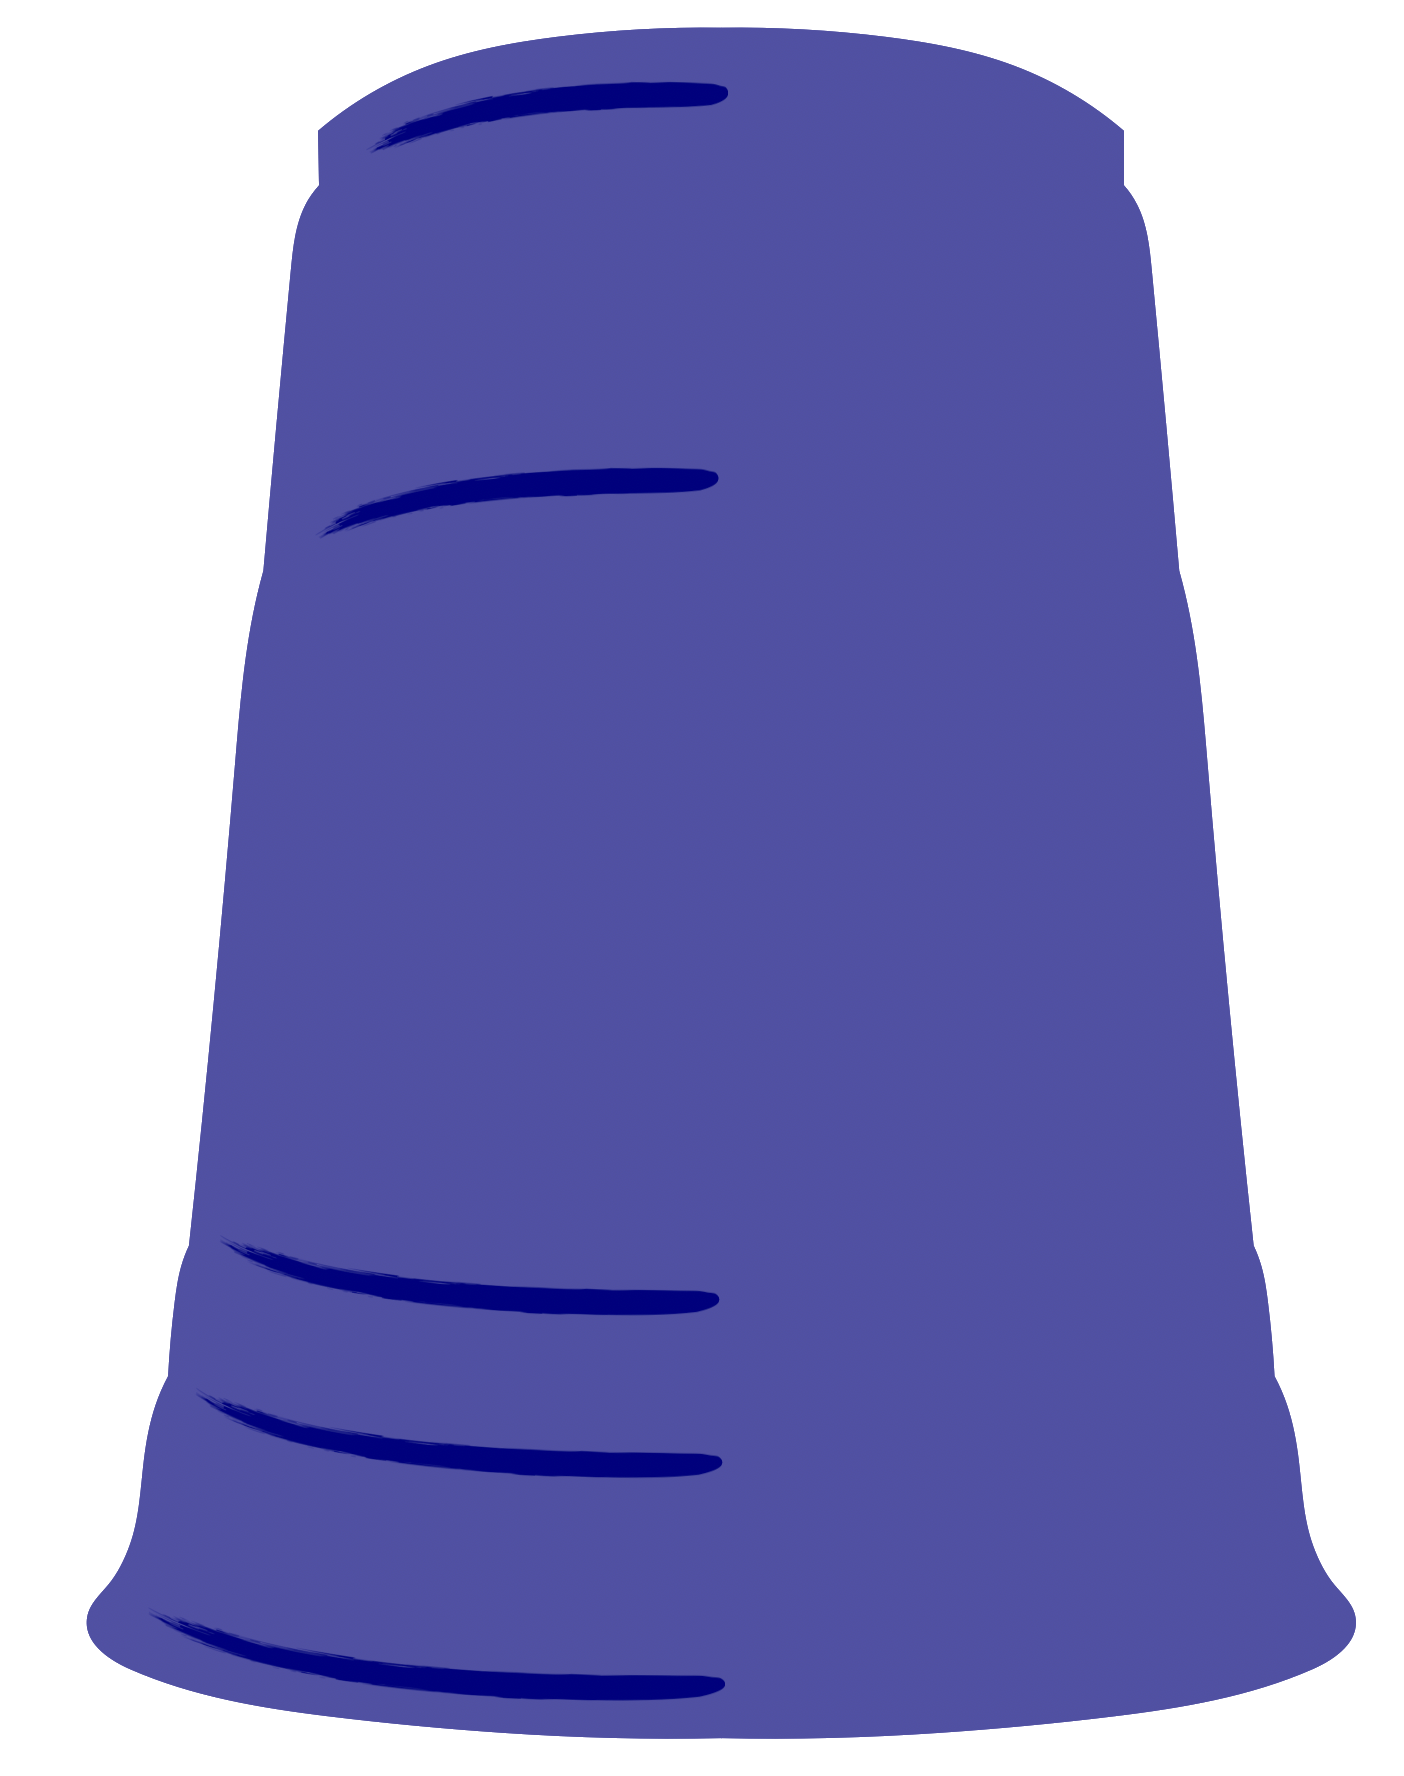
\includegraphics[width=2cm]{cup_down.png}};

				\begin{scope}[scale=0.7, shift={(-17, 3)}, rotate=-5]
					\fill[dark, rounded corners=3] (0, 0) rectangle (10, 6);
					\fill[black] (0, 0.5) rectangle (10, 3.5);
					\node[text=white, align=center, rotate=-5] at (5, 5.2) { \small \textsf{HELLO} };
					\node[text=white, align=center, rotate=-5] at (5, 4.1) { \tiny \textsf{my name is } };
					\node[text=white, align=center, rotate=0] at (5.25, 2) { \large \textsl{Group 3} };
				\end{scope}

				\fill[dark] (0, 4) circle (1);
				\node at (0, 7) {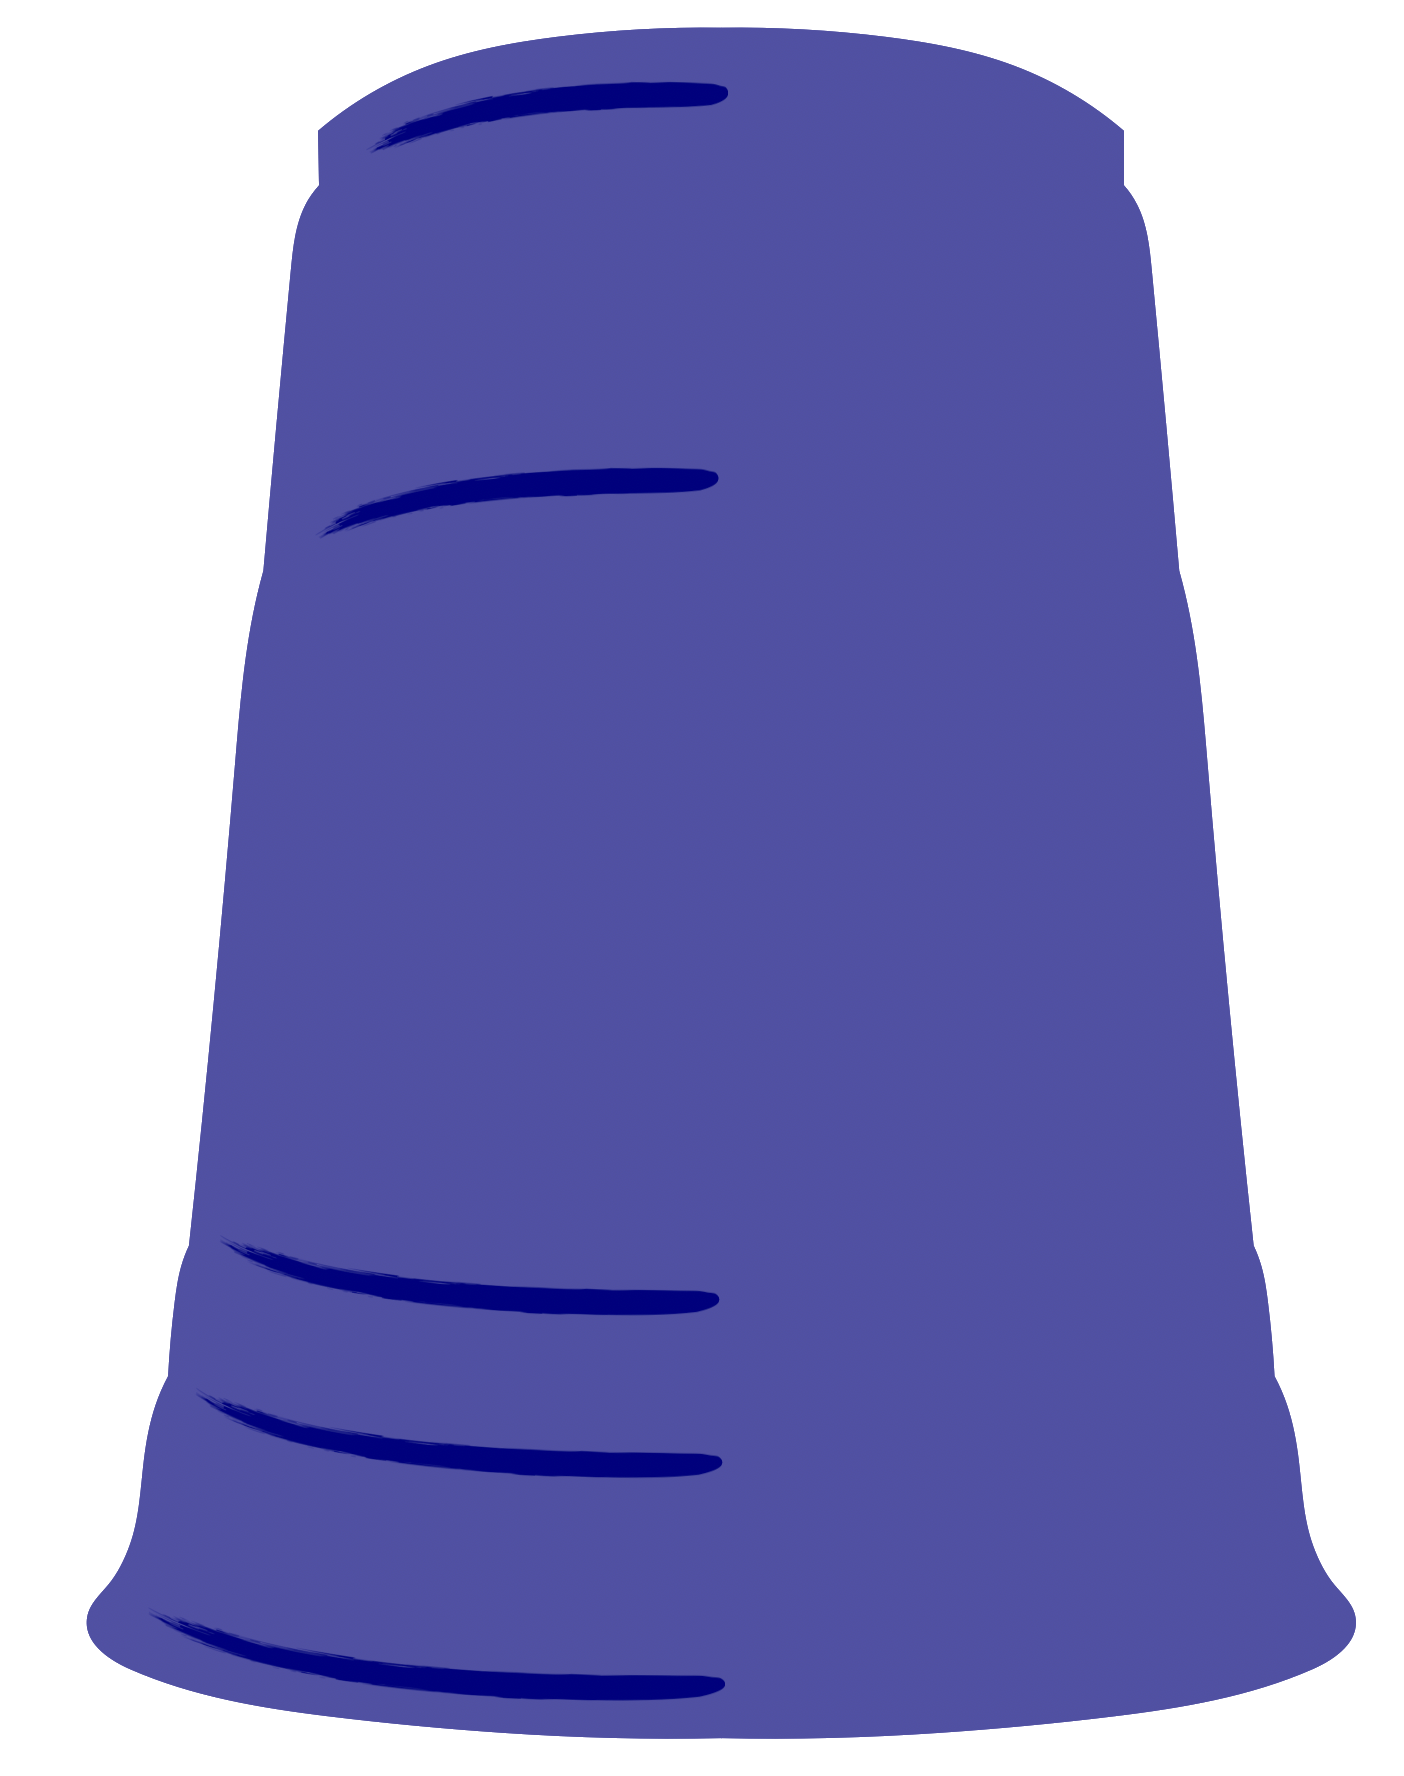
\includegraphics[width=2cm]{cup_down.png}};

				\begin{scope}[scale=0.7, shift={(-2, 3)}, rotate=10]
					\fill[dark, rounded corners=3] (0, 0) rectangle (10, 6);
					\fill[black] (0, 0.5) rectangle (10, 3.5);
					\node[text=white, align=center, rotate=10] at (5, 5.2) { \small \textsf{HELLO} };
					\node[text=white, align=center, rotate=10] at (5, 4.1) { \tiny \textsf{my name is } };
					\node[text=white, align=center, rotate=7] at (5.25, 2) { \large \textsl{Group 1} };
				\end{scope}

				\fill[dark] (+10, 4) circle (1);
				\node at (+10, 7) {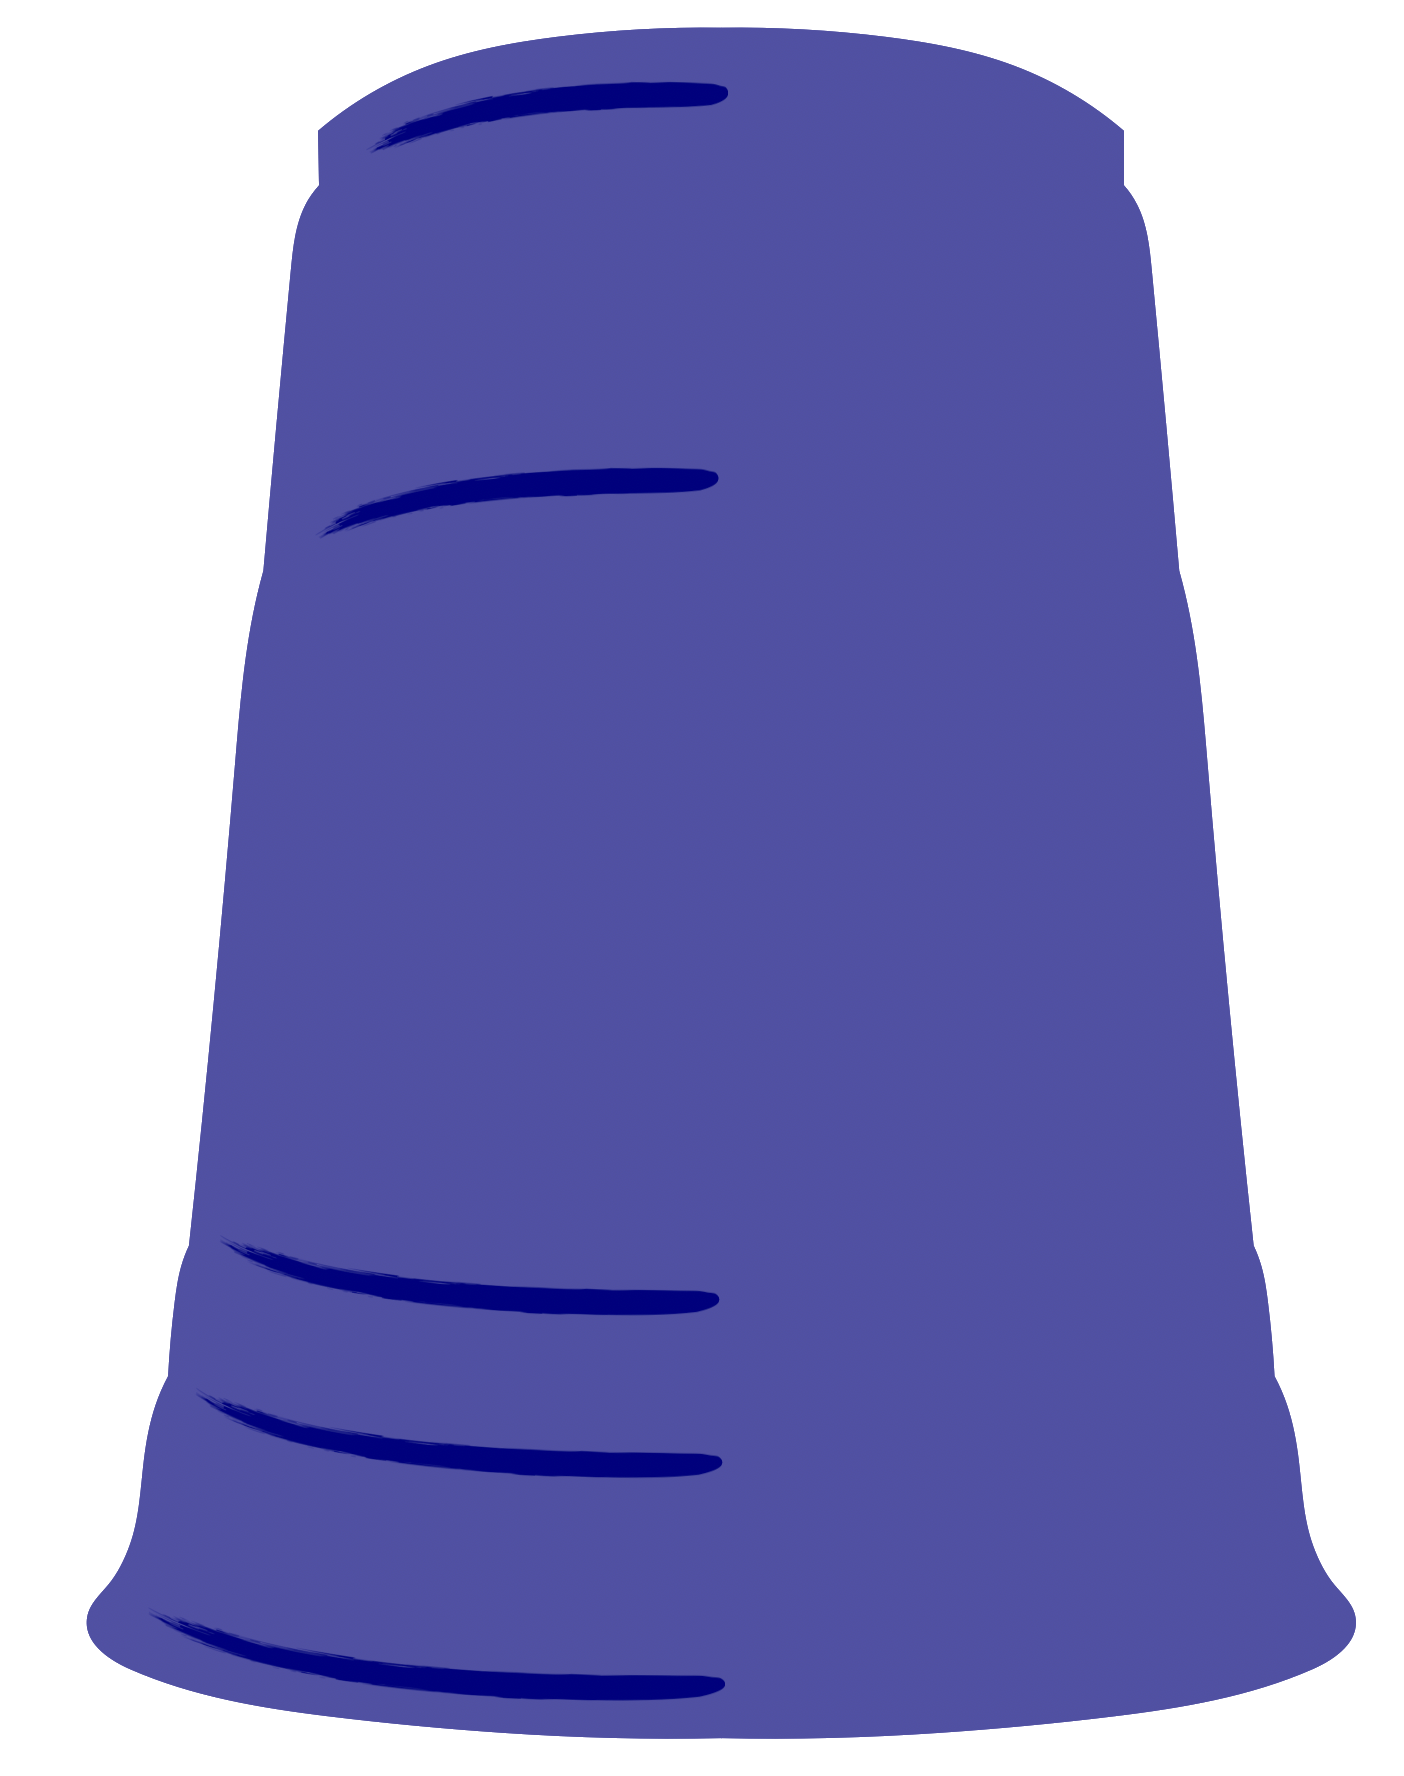
\includegraphics[width=2cm]{cup_down.png}};

				\begin{scope}[scale=0.7, shift={(12, 3)}, rotate=1]
					\fill[dark, rounded corners=3] (0, 0) rectangle (10, 6);
					\fill[black] (0, 0.5) rectangle (10, 3.5);
					\node[text=white, align=center, rotate=1] at (5, 5.2) { \small \textsf{HELLO} };
					\node[text=white, align=center, rotate=1] at (5, 4.1) { \tiny \textsf{my name is } };
					\node[text=white, align=center, rotate=1] at (5.25, 2) { \large \textsl{Group 2} };
				\end{scope}

				\draw[light, <->, >=stealth, line width=4]
				(-8, 6.5) .. controls (-7, 7.5) and (-6.5, 8.25) ..
				(-4.5, 8.5) .. controls (-2.5, 8.75) and (-1, 8.5) .. (0, 7);
				\draw[dark, <->, >=stealth, line width=2]
				(-7.85, 6.65) .. controls (-7, 7.5) and (-6.5, 8.25) ..
				(-4.5, 8.5) .. controls (-2.5, 8.75) and (-1, 8.5) .. (-0.15, 7.15);

				\draw[light, <->, >=stealth, line width=4]
				(3, 7.5) .. controls (4, 9) and (6.25, 9.75) ..
				(8.25, 9.5) .. controls (10.25, 9.25) and (11, 8.75) .. (12, 6.75);
				\draw[dark, <->, >=stealth, line width=2]
				(3.15, 7.65) .. controls (4, 9) and (6.25, 9.75) ..
				(8.25, 9.5) .. controls (10.25, 9.25) and (11, 8.75) .. (11.9, 6.9);

				\draw[light, <->, >=stealth, line width=4]
				(-8, 1.5) .. controls (-7, -1.5) and (2, -1.25) ..
				(4, -1) .. controls (6, -0.75) and (11, -0.5) .. (12, 1.5);
				\draw[dark, <->, >=stealth, line width=2]
				(-7.925, 1.25) .. controls (-7, -1.5) and (2, -1.25) ..
				(4, -1) .. controls (6, -0.75) and (11, -0.5) .. (11.9, 1.3);

			\end{scope}

		\end{tikzpicture}
	\end{adjustbox}
\end{frame}

\subsection{Hyperprior}
\begin{frame}{Hyperprior}
	In hierarchical models, we have a hyperprior,
	which is a prior's prior:
	$$
		\begin{aligned}
			\mathbf{y}        & \sim \text{Normal}(10, \boldsymbol{\eta}) \\
			\boldsymbol{\eta} & \sim \text{Normal}(0, \omega)             \\
			\omega            & \sim \text{Normal}^+(1)
		\end{aligned}
	$$
	Here $\mathbf{y}$ is a variable of interest that belongs to distinct groups.
	$\boldsymbol{\eta}$, a prior for $\mathbf{y}$,
	is a vector of group-level parameters with their own prior
	(which becomes a hyperprior) $\omega$.
\end{frame}

\subsection{Mathematical Specification of Hierarchical Models}
\begin{frame}{Mathematical Specification of Hierarchical Models}
	We have $N$ observations organized in $J$ groups with $K$ covariates.
	$$
		\begin{aligned}
			\mathbf{y}          & \sim \text{Normal}(\mathbf{X} \boldsymbol{\eta_{j}}, \sigma)                                                       \\
			\boldsymbol{\eta_j} & \sim \text{Multivariate Normal}(\mathbf{0}, \boldsymbol{\Omega})
			\quad \text{for}\quad j \in \{ 1, \dots, J \}                                                                                            \\
			\boldsymbol{\Omega} & = \operatorname{Diagonal}(\boldsymbol{\omega}) \cdot \mathbf{C} \cdot \operatorname{Diagonal}(\boldsymbol{\omega}) \\
			\boldsymbol{\omega} & \sim \text{Normal}(0, 0.4)                                                                                         \\
			\mathbf{C}          & \sim \text{LKJ}(\eta)                                                                                              \\
			\sigma              & \sim \text{Exponential}(1)
		\end{aligned}
	$$
	Each coefficient vector $\boldsymbol{\eta}_j$ represents the
	model columns $\mathbf{X}$ coefficients for every group $j \in J$.
\end{frame}

\begin{frame}{Mathematical Specification of Hierarchical Models}
	If you need to extend to more than one group,
	such as $J_1, J_2, \dots$:
	$$
		\begin{aligned}
			\mathbf{y}             & \sim \text{Normal}(\alpha + \mathbf{X} \boldsymbol{\eta_{j1}} + \mathbf{X} \boldsymbol{\eta_{j2}}, \sigma)               \\
			\boldsymbol{\eta_{j1}} & \sim \text{Multivariate Normal}(\mathbf{0}, \boldsymbol{\Omega}_1)
			\quad \text{for}\quad j_1 \in \{ 1, \dots, J_1 \}                                                                                                 \\
			\boldsymbol{\eta_{j2}} & \sim \text{Multivariate Normal}(\mathbf{0}, \boldsymbol{\Omega}_2)
			\quad \text{for}\quad j_2 \in \{ 1, \dots, J_2 \}                                                                                                 \\
			\boldsymbol{\Omega_1}  & = \operatorname{Diagonal}(\boldsymbol{\omega_1}) \cdot \mathbf{C_1} \cdot \operatorname{Diagonal}(\boldsymbol{\omega_2}) \\
			\boldsymbol{\Omega_1}  & = \operatorname{Diagonal}(\boldsymbol{\omega_1}) \cdot \mathbf{C_2} \cdot \operatorname{Diagonal}(\boldsymbol{\omega_2}) \\
			\mathbf{C_1}           & \sim \text{LKJ}(\eta_1)                                                                                                  \\
			\mathbf{C_2}           & \sim \text{LKJ}(\eta_2)                                                                                                  \\
			\sigma                 & \sim \text{Exponential}(1)
		\end{aligned}
	$$
\end{frame}
